In this chapter we will go through how the installations have been analysed and present the findings. Then we will revisit the theoretical framework and reflect on the generated knowledge from the practical application of the framework.

\section{Systematising the installations}
Over the course of this thesis, my research buddies and I have visited seven exhibitions from 4 local museums in Oslo, (Table 7.1). Two of the exhibitions took place at the University of Oslo: department of informatics (ifi), as part of the course Tangible Interaction (IN5470). From these museum visits, we have documented 21 interactive installations that make up the data set, see Table 7.2 for listing of the installations. In the following sections, we will see how the theoretical framework has been applied, e.g., Tables 7.3, 7.4, 7.8, to the resulting Findings Table 7.9, in section 7.5. Note that all installations are sorted in the same numeric order as in Table 7.2: Installations, meaning that the numbering in Table 7.2 numerically identifies the installation following the analysis in all tables.

\begin{table}[H]
\centering
\begin{tabular}{| l | l| l|}
\hline
\textbf{Type} & \textbf{Name} & \textbf{Museum}\\
\hline
Exhibition & Vi står i det nå & Klimahuset \\
Exhibition & I/O (In Oslo) & Atelier Nord\\
Exhibition & Shadows & MUNCH\\
Exhibition & Poison & MUNCH \\
Exhibition & Input/Output & Teknisk Museum \\
Exhibition & Slow Design: reveal & ifi \\
Exhibition & Haptic Interaction & ifi \\
\hline
\end{tabular}
\caption{Exhibitions}
\label{tab:abc}
\end{table}

\begin{table}[H]
\centering
\begin{tabular}{| l | l | l|}
\hline
\textbf{Nr} & \textbf{Exhibition} & \textbf{Installation}\\
\hline
1 & Input/Output & Input/Output  \\
2 & I/O (In Oslo) & I/O (In Oslo)\\
3 & Slow Design & Qi \\
4 & Slow Design & Memento Mori \\
5 & Slow Design & Presence in existence \\
6 & Haptic Interaction & The Maze \\
7 & Haptic Interaction & Black Horizon \\
8 & Haptic Interaction & The unfair fun fair \\
9 & Vi står i det nå & Crank lever \\
10 & Vi står i det nå & Rotating disc \\
11 & Vi står i det nå & Solutions \\
12 & Vi står i det nå & Video theatre \\
13 & MUNCH & Shadows -- Paint like Munch \\
14 & MUNCH & Shadows -- Resting sofa chair  \\
15 & MUNCH & Shadows -- Camera \\
16 & MUNCH & Shadows -- Edvard M. paints your portrait  \\
17 & MUNCH & Shadows -- Radio \\
18 & MUNCH & Shadows -- Telephone  \\
19 & MUNCH & Shadows -- Suitcases  \\
20 & MUNCH & Shadows -- Housekeeper  \\
21 & MUNCH & Poison  \\
\hline
\end{tabular}
\caption{Installations}
\label{tab:abc}
\end{table}


\section{Application of theoretical framework}
In my attempt to answer how one can design meaningful interactive experiences in a museum space that addresses sustainability, I have accounted for three place-centred approaches that I base my understanding of meaningfulness on; \emph{Hybrid place, place as a dialogue} and \emph{Sense-making strategies}. As is accounted for in Chapter 4: A new way of designing for meaningfulness?. The aim is that the framework provides a theoretically grounded but practical way for the designer to identify meaningful relations between visitor-experience, installation and the museum, in a museum or exhibition space. The challenge of combining/ putting the three approaches together is that we end up with 14 different parameters; e.g. social and cultural dimension from the \emph{Hybrid Place} framework, vs open, and, situates artefact in narrative principle from \emph{Place as a Dialogue}. To see how this would play out, it was decided to make one table for each theory, where each installation is categorised up against the four or five principles. This would help us get a feeling of how the theory would apply to the data-set (installation) in practise. In addition it was made a radar-chart as a complementing way of interpreting the data-set. See section 7.3: Tables and Radar Charts, Table 7.3-7.8 for the tables and radar charts. This way we could first learn how applicable the different principles/ or dimensions are for the data-set for each respective theory, and secondly open for seeing connections across/ between the theories; "the bigger picture". The tables later also proved useful as quick-reference guides when mapping out the findings. The categorisation of the data is highly subjective but theoretically grounded, based on my personal experience with- and interpretation of the installations and knowledge of the museum institution the installation was part of. The plotting of the tables are based upon the written experience accounts and my subjective intuition consisting of both my memory and take-away of the installation. In a pilot analysis session I chose to merge all of the MUNCH - \emph{Shadows} installations as one, because I did not think they differed enough in their interactive qualities, and I was afraid that they were going to skew the data. Because of this, the data-set shrinked from 21 to 16 installations in total. After the first categorisation where the MUNCH \emph{shadows} installations was counted as one, I wanted to compare and see what happened when I categorised each \emph{Shadows} installation. Going through the \emph{Shadows} installations once again, it became clear that they did not all "check the same boxes", which strengthened the decision to count them separately. Then, the data-set increased back to 21 installations in total. The framework's practical application also generate three radar charts, where the dimensions/ principles make up the edges of the radar chart, and the numbered lines outward represent the number of installations. E.g. in Figure 7.4, you can see the number of installations starting from 0 in the centre up to 17 outermost. That tell us that of 21 installations in total, 17 of is the highest amount of installations that count that specific dimension/ principle.

Next we present a visualisation, Figure 7.1, that aim to illustrate how each theory contribute to the understanding of meaningfulness. The lines represents what we strive to find; dialogic relations between visitor and installation, while the tables help to objectify three aspects related to this thesis understanding of meaningfulness as a discourse demanding support and extension of conversations, reflections and augmented experiences. Supported and extended through interactive qualities, which is how we propose an objectification of meaningfulness as a quality that you can design for, in the scope of this research context and design space. Then we will present the Tables and radar charts, with a short description of what we can see and learn from them.

\begin{figure}[H]
\centering
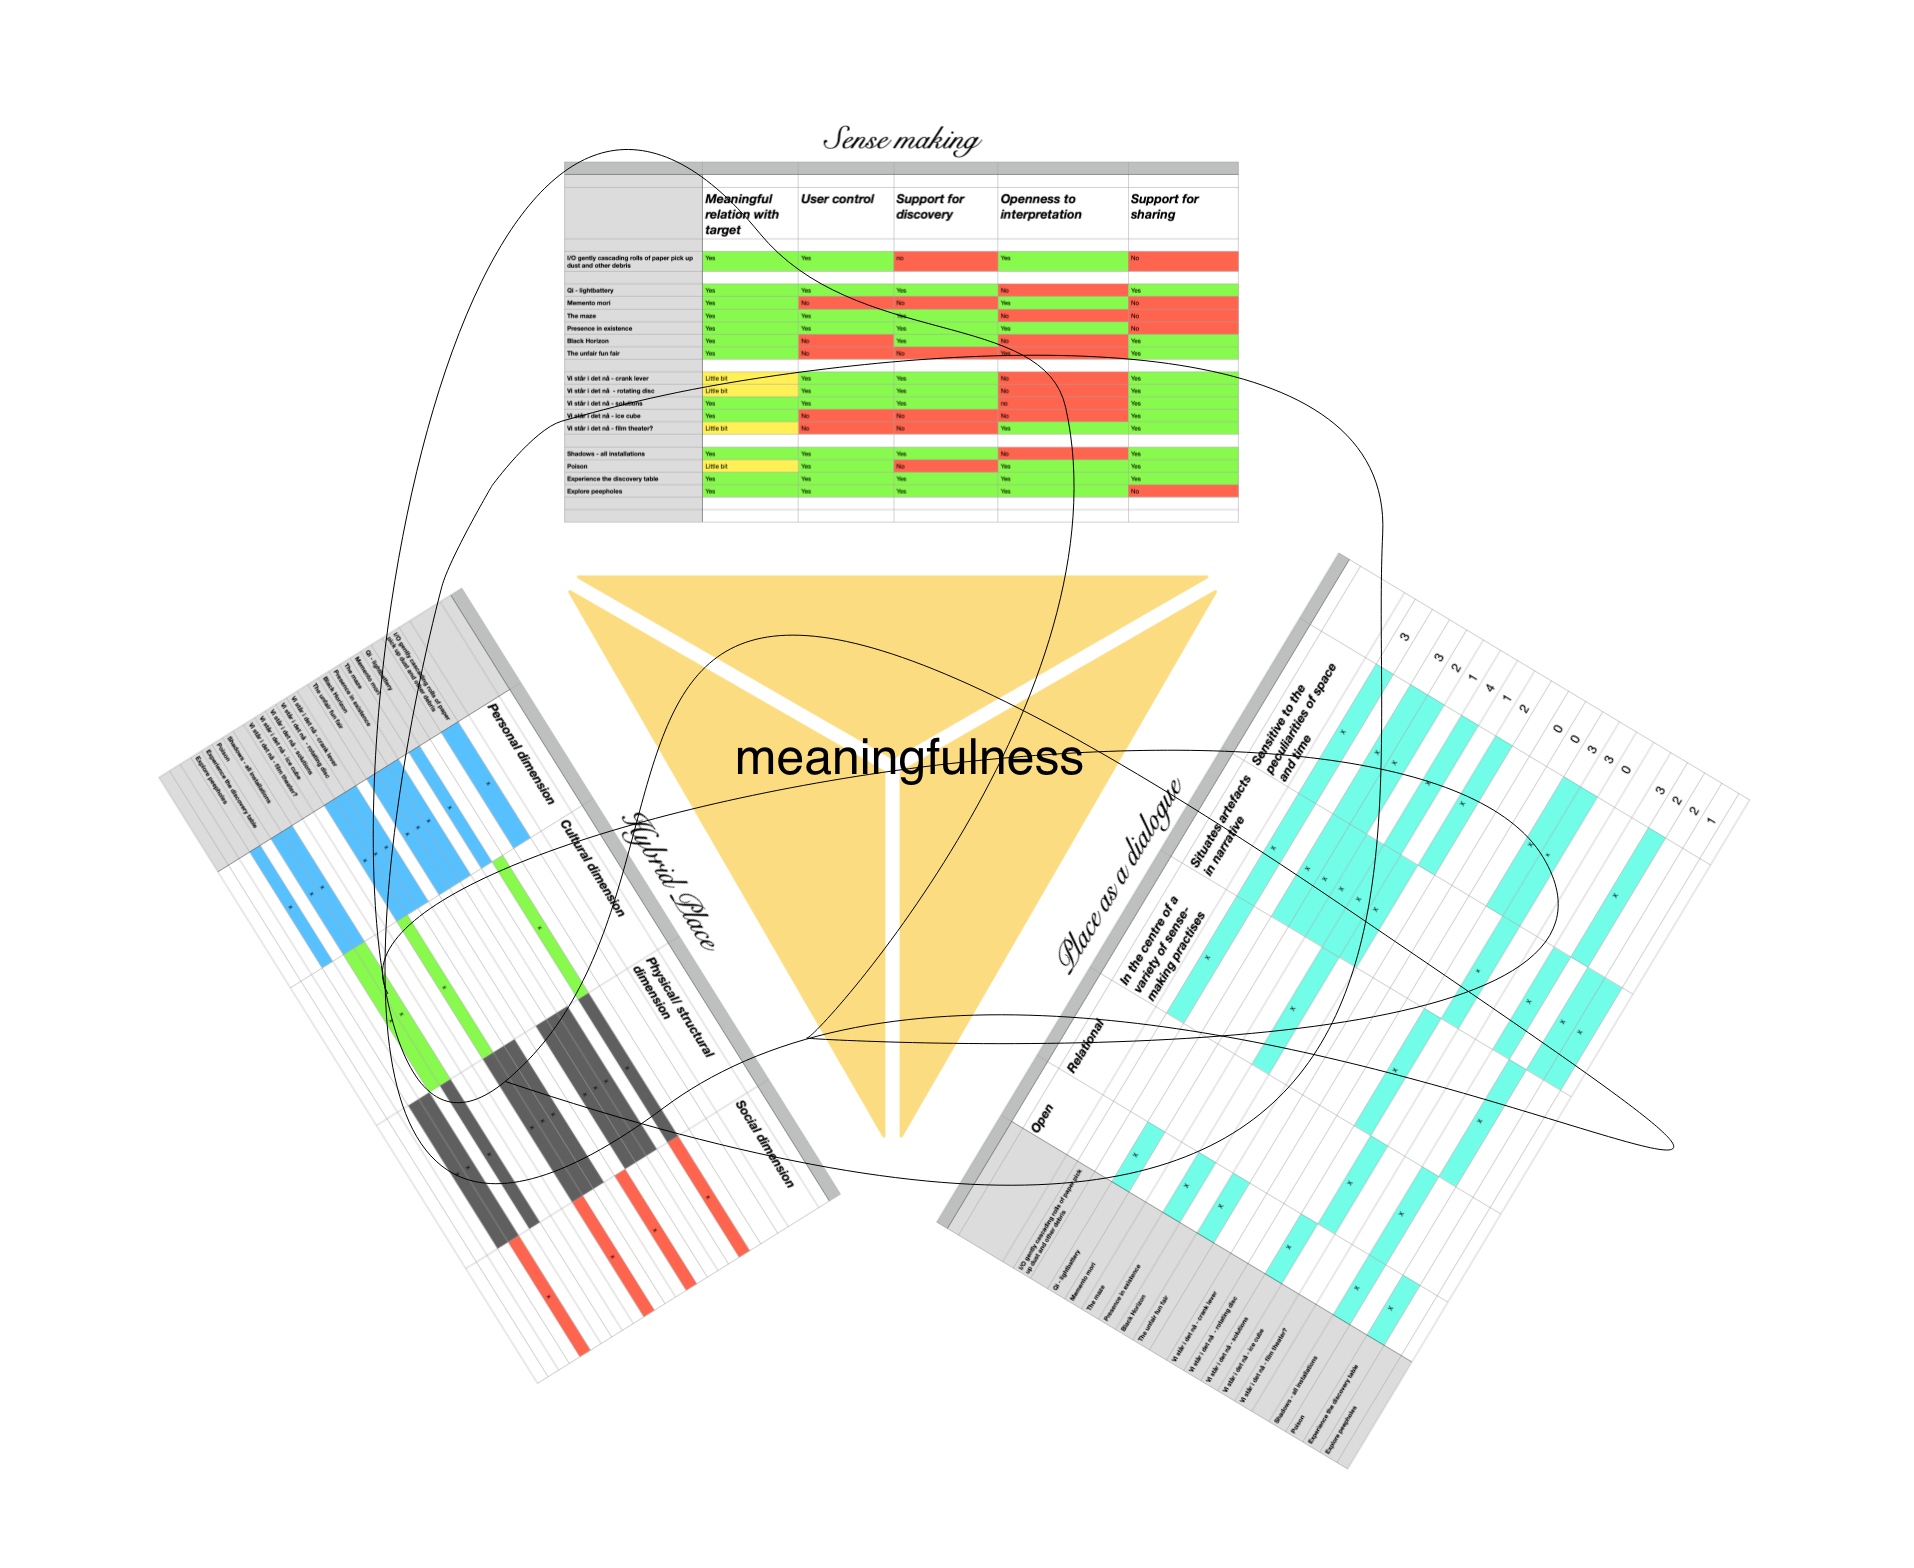
\includegraphics[width=15cm]{pictures/analysis/table_triangle.png}
\caption{Framework of Meaningfulness}{This visualisation aim to illustrate how each theory contribute to the understanding of meaningfulness. The lines in-between the triangle and tables represents dialogic relations between visitor and installation, while the tables objectify three aspects related to meaningfulness.}
\end{figure}

\section{Tables and Radar Charts}

\begin{table}[H]
    \centering 
    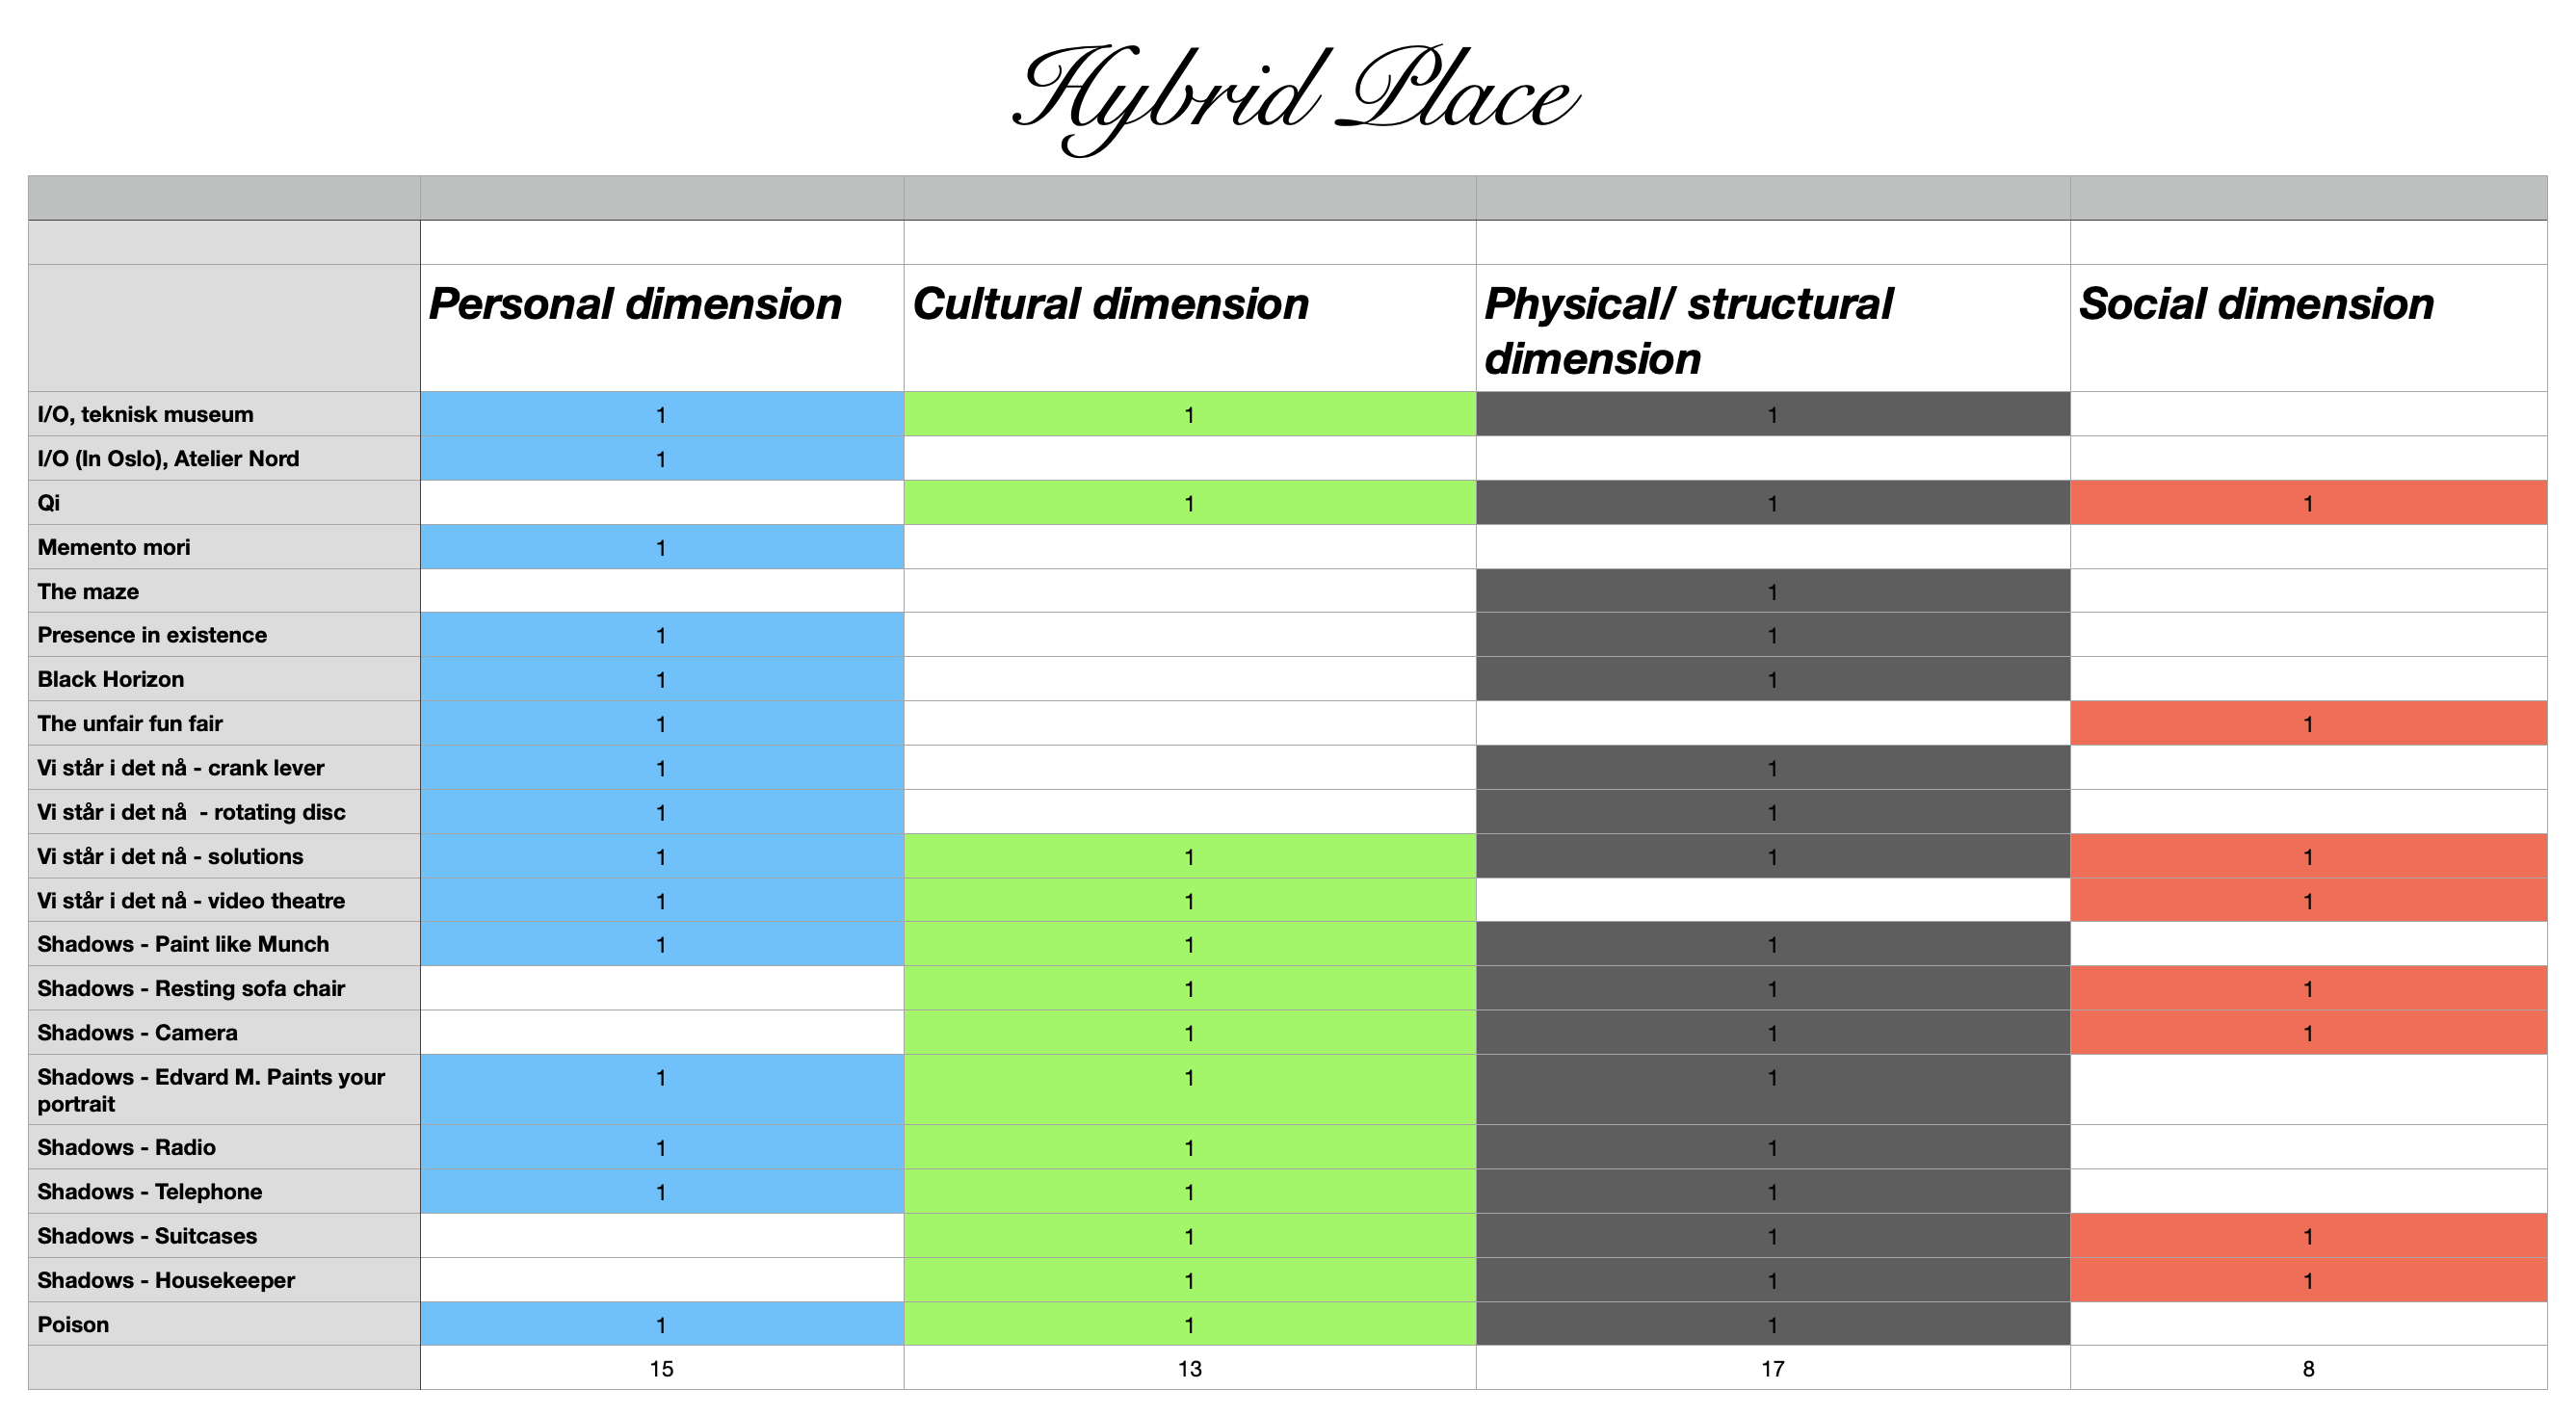
\includegraphics[width=20cm, angle=90]{pictures/analysis/hybrid.png}
    \caption{Hybrid Place table}
\end{table}

\begin{table}[H]
    \centering 
    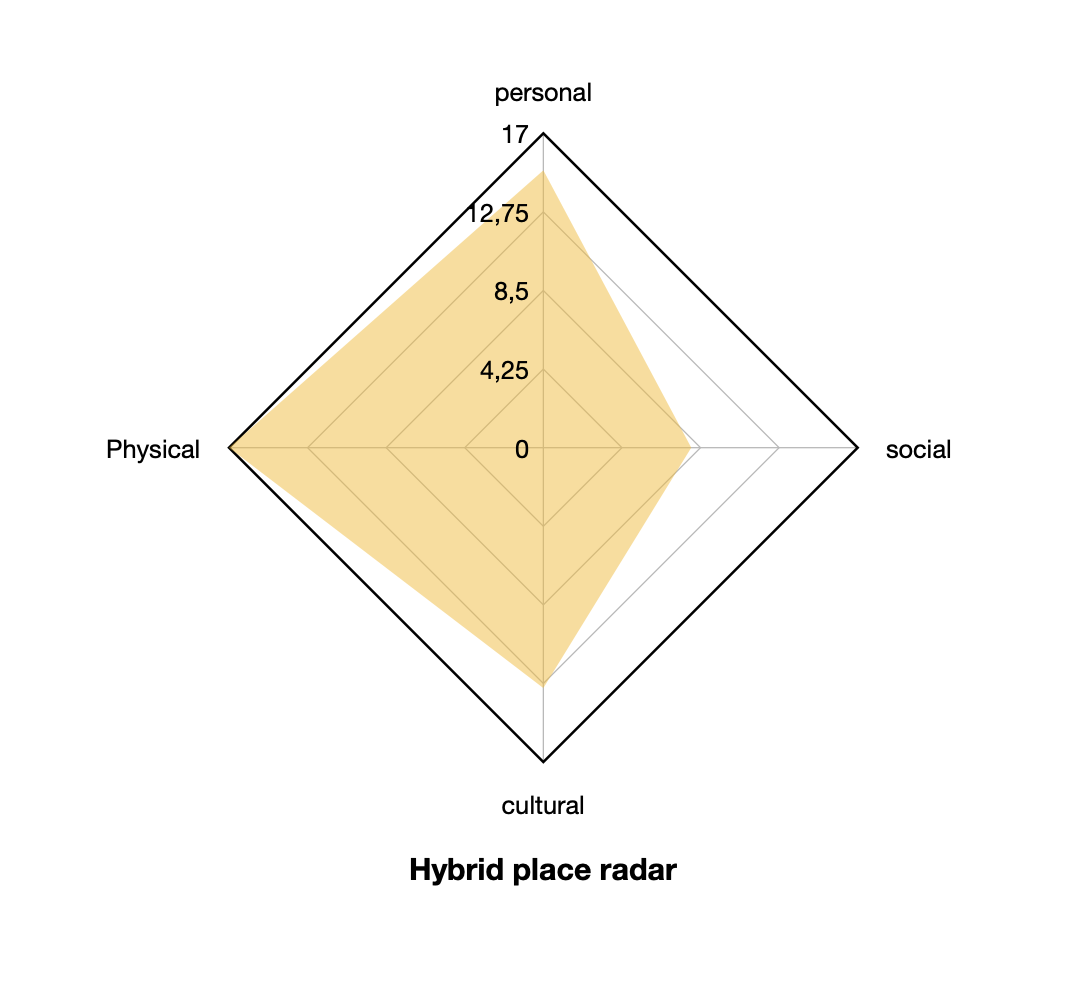
\includegraphics[width=12.5cm]{pictures/analysis/hybrid_radar.png}
    \caption{Hybrid Place radar}
\end{table}


From the radar chart 7.4 we can see that the \textit{Physical} counting 17 installations and \textit{Personal} counting 15 installations being the most weighted dimensions. The \textit{Cultural} dimension less so, and the \textit{Social} dimension the least, counting 8. Comparing with Table 7.3, we see that the MUNCH \textit{Shadows} installations account for both the Physical and Cultural dimension results to stand out, whereas all of Shadows marks Cultural and Physical and therefore can pose a risk of skewing the data. Looking at Table 7.3 again, we can see that the Physical dimension still would be weighted along with the Personal dimension if we were to see MUNCH \textit{Shadows} as one, whereas the Cultural would count only four installations if we were to remove the MUNCH \emph{Shadows} installations.

\begin{table}[H]
    \centering 
    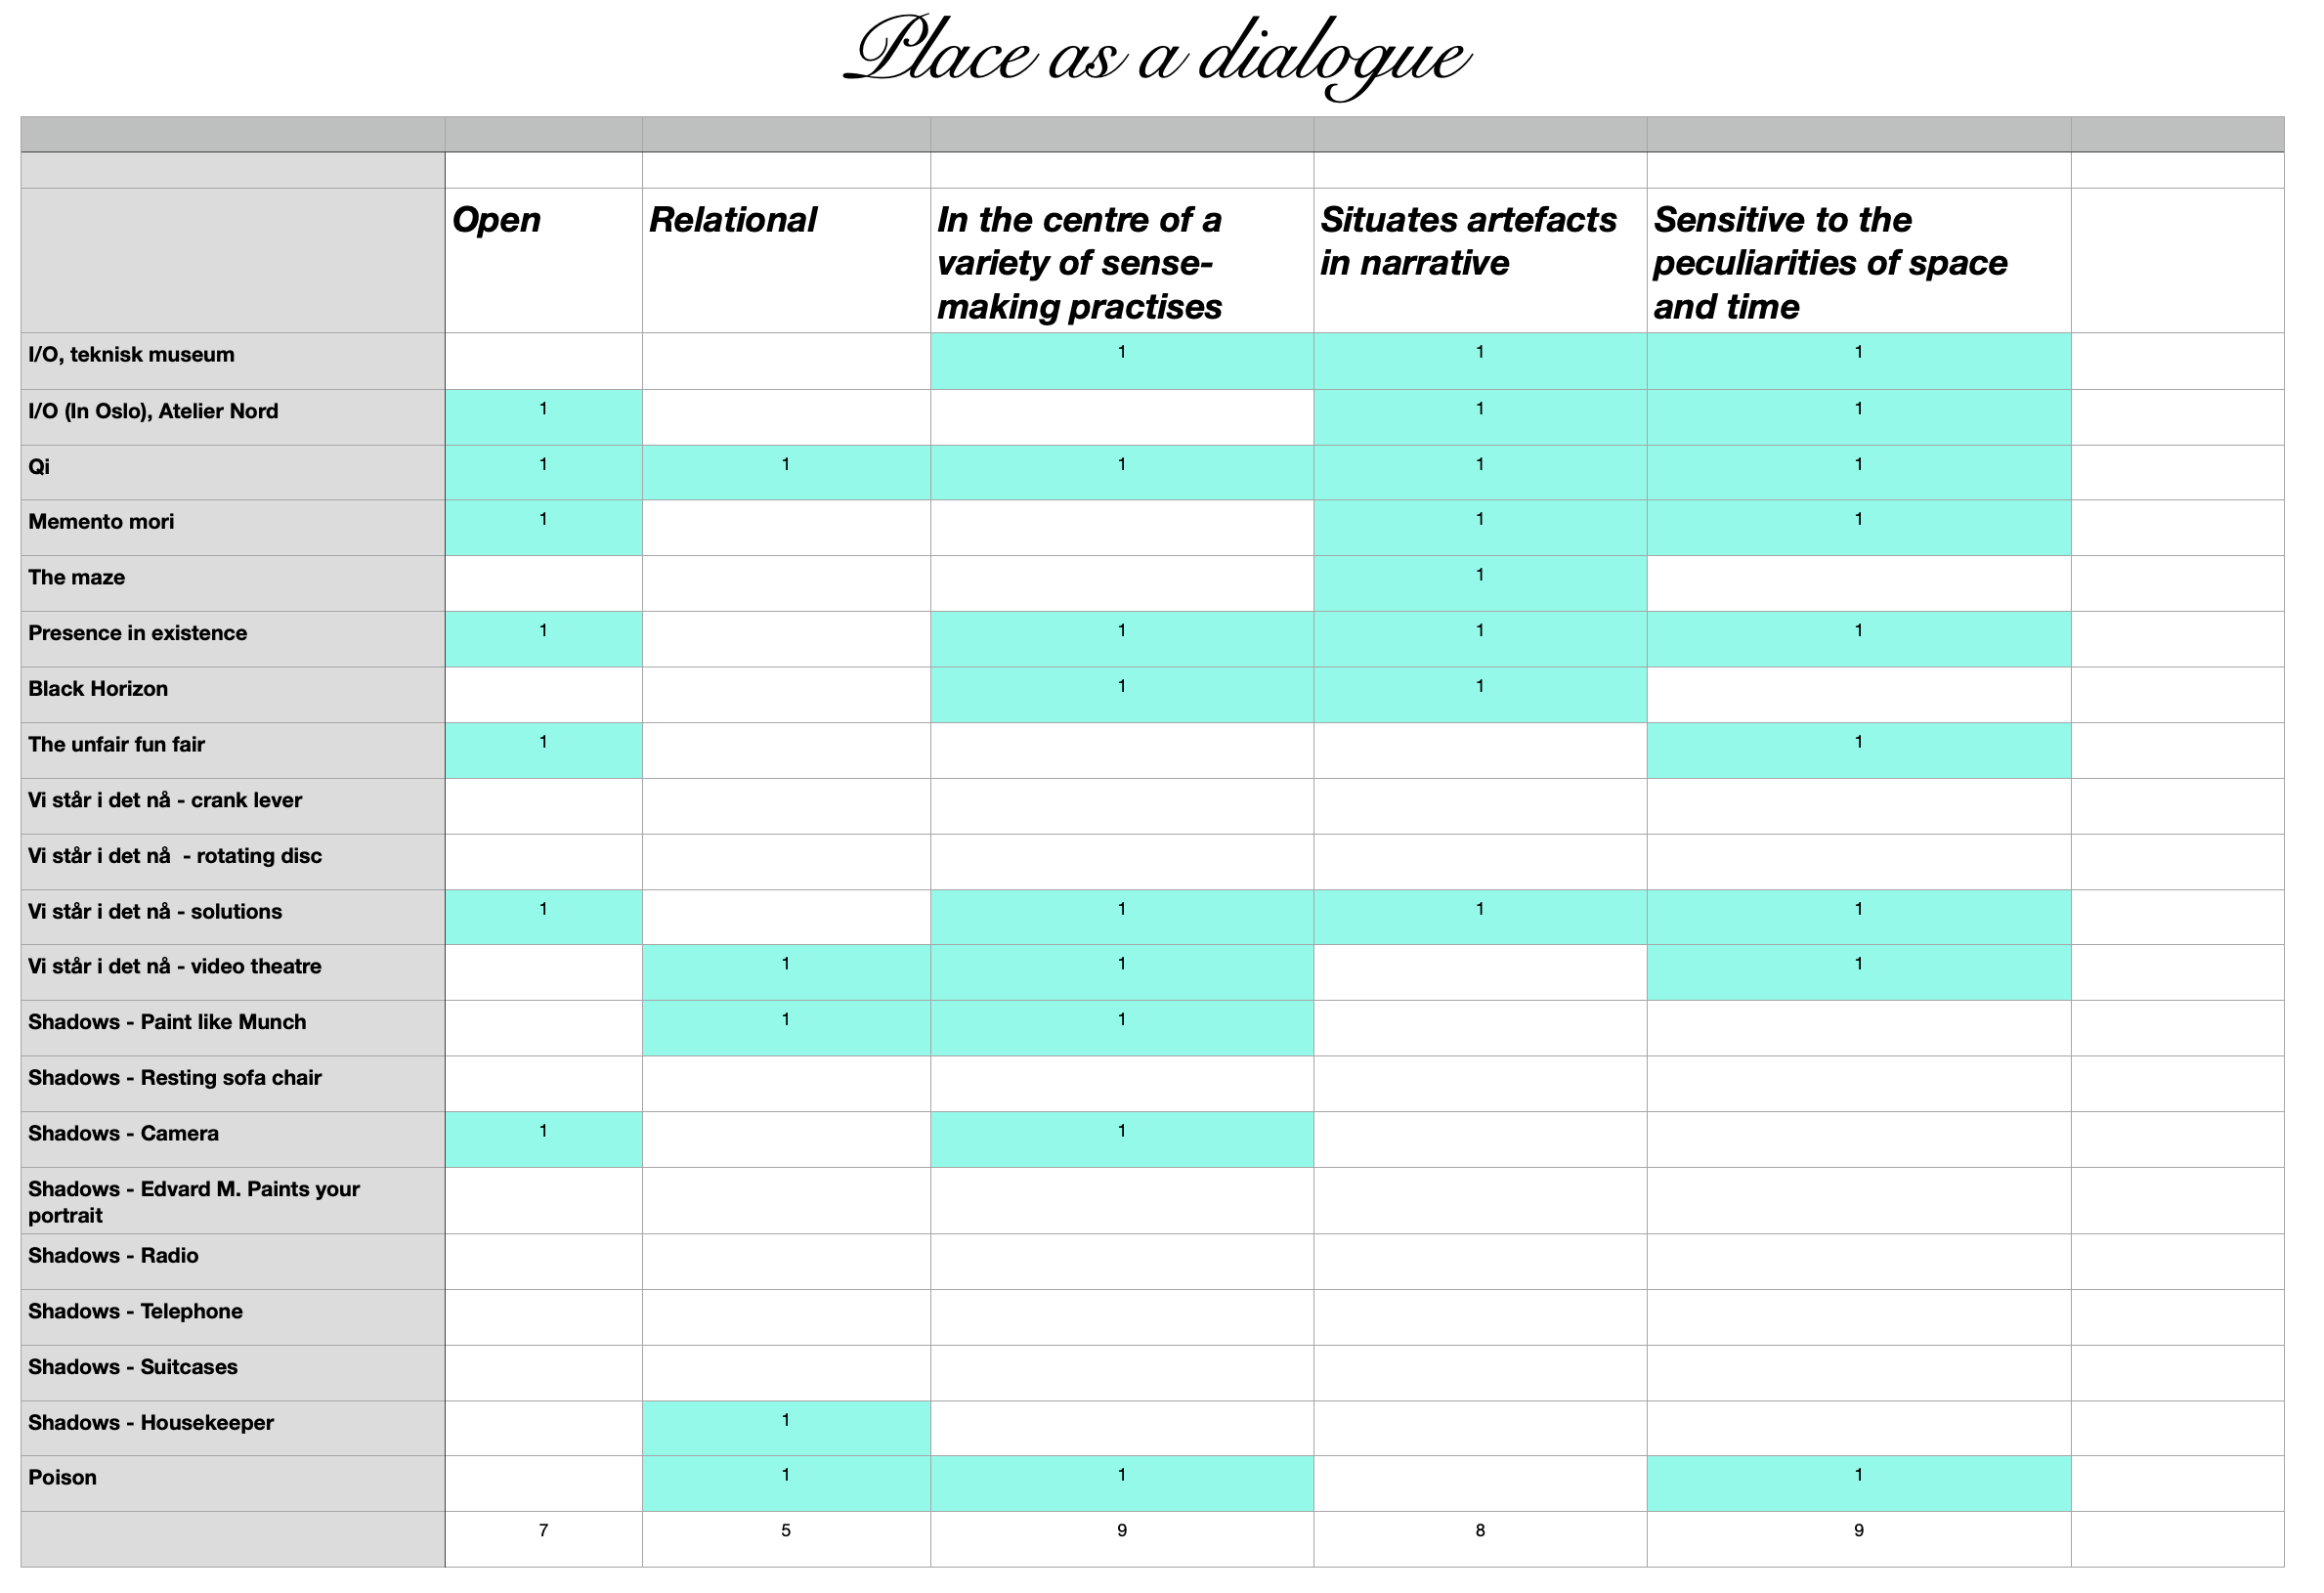
\includegraphics[width=20cm, angle=90]{pictures/analysis/place.png}
    \caption{Place as a Dialogue table}
\end{table}

\begin{table}[H]
    \centering 
    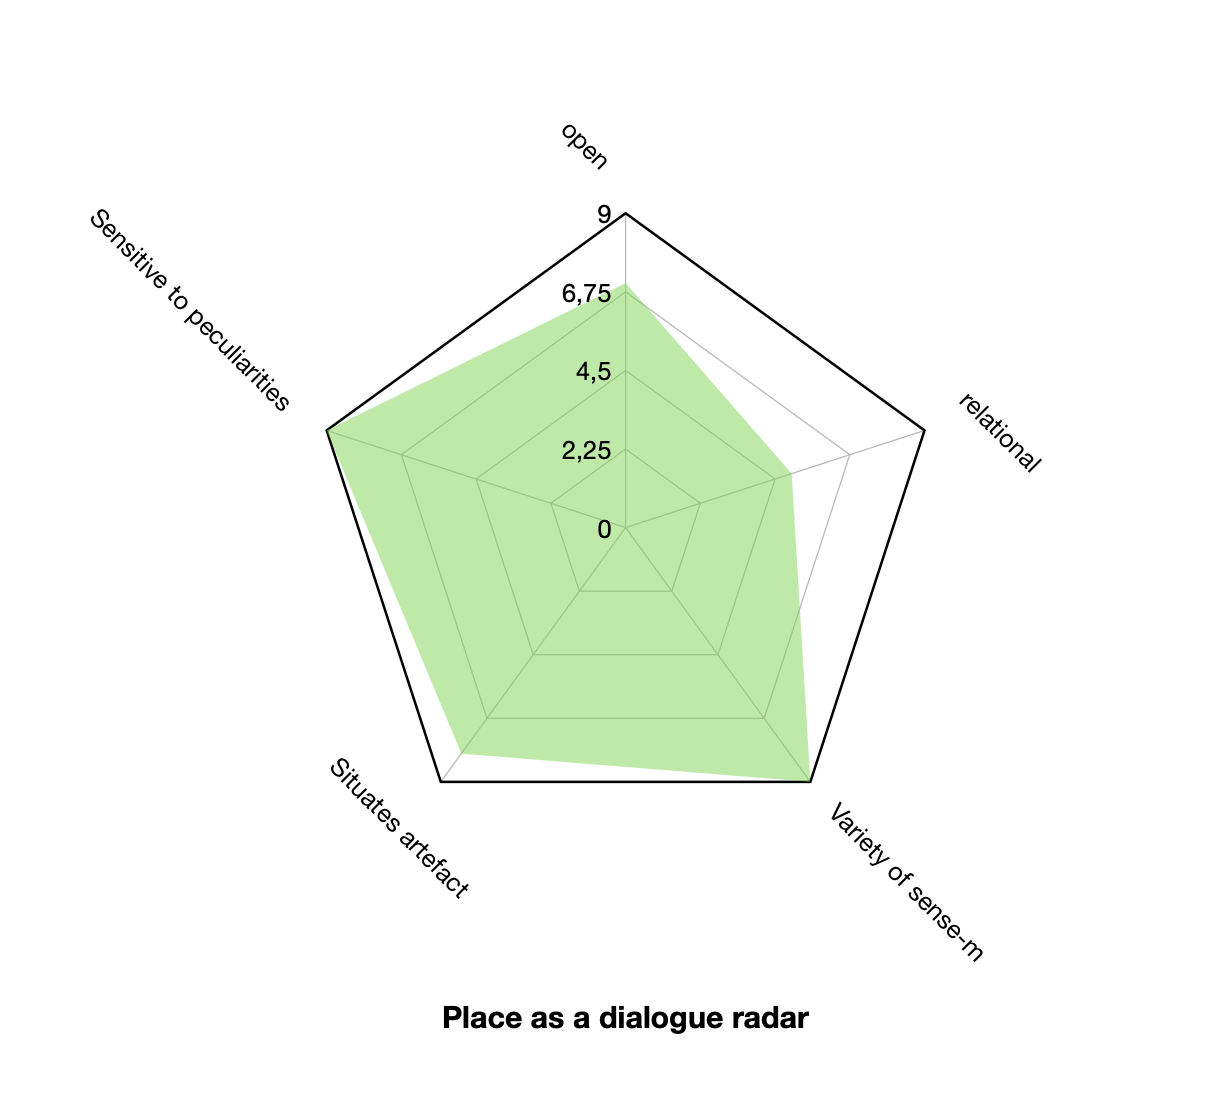
\includegraphics[width=12.5cm]{pictures/analysis/place_radar.png}
    \caption{Place as a Dialogue radar}
\end{table}


From the radar chart 7.6, we can see that the installations point to \textit{Situates artefact in narrative} as the most fulfilled by counting 15 installations. While \textit{Open}, \textit{In the centre of a variety of sense-making practises}, \textit{Sensitive to peculiarities of space and time}, are all moderately weighted. While \textit{Relational} are the least fulfilled principle, counting 6 installations. Except for one other installation, there is only MUNCH \emph{Shadows} who fulfill the relational principle, again at risk of skewing the data-set trend. In terms of the most fulfilled principle, \emph{situates artefact in narrative}, the installations that do not fulfill the principle are the ones where the visitor itself is situated in the narrative.


\begin{table}[H]
    \centering 
    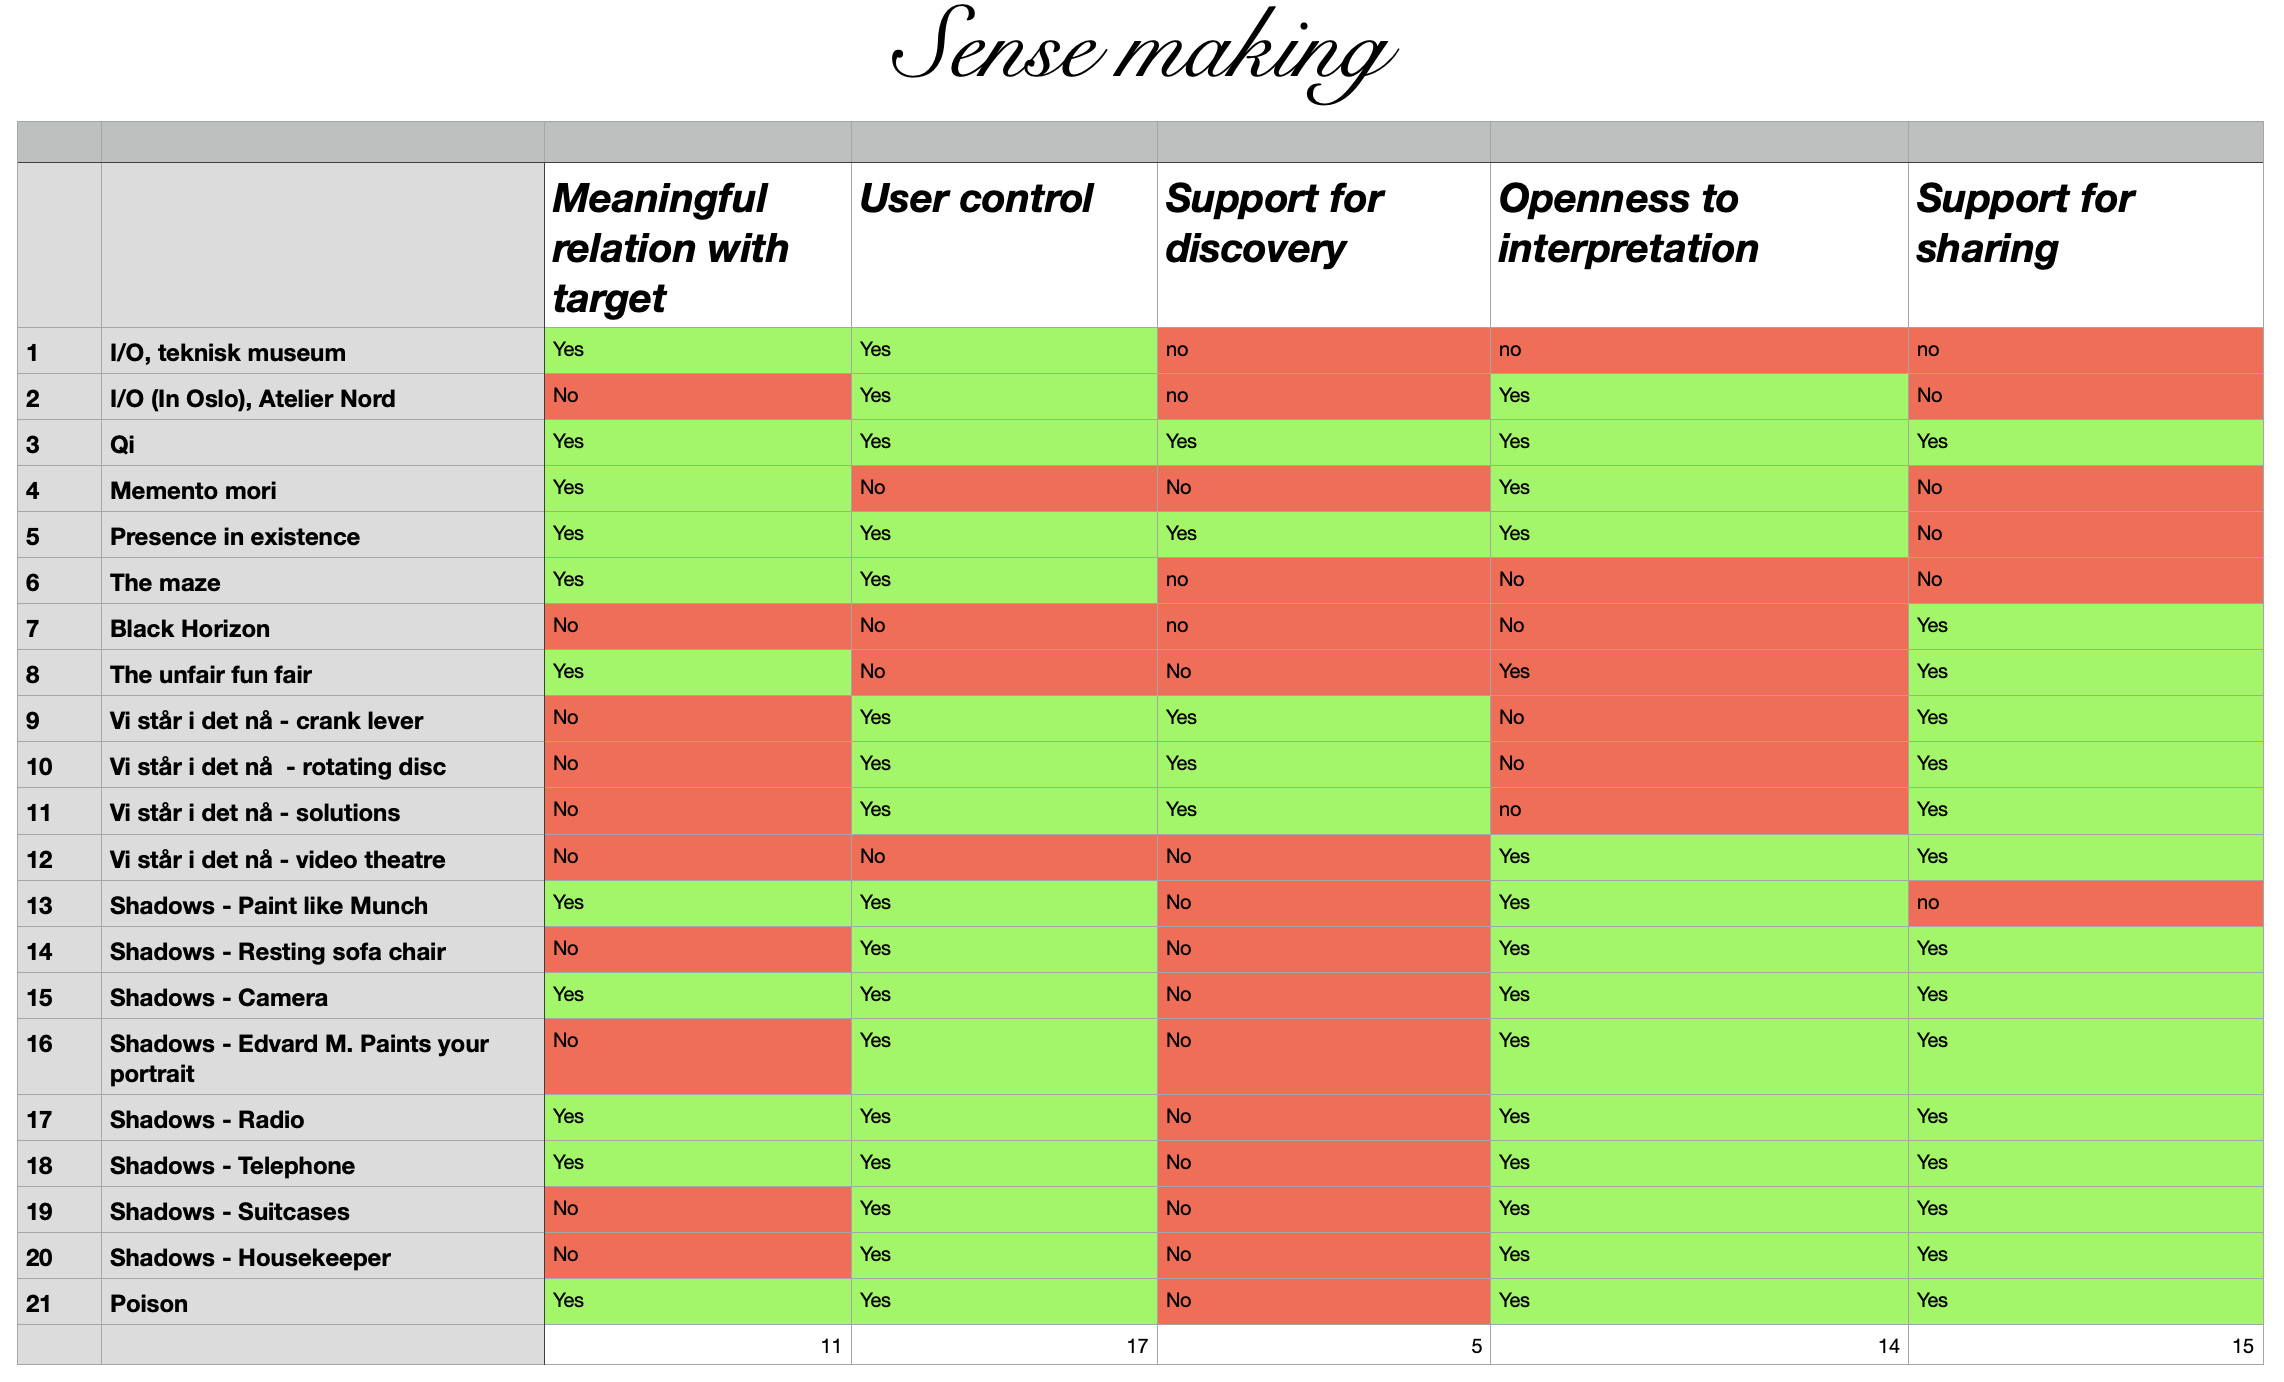
\includegraphics[width=20cm, angle=90]{pictures/analysis/sense.png}
    \caption{Sense-making table}
\end{table}

\begin{table}[H]
    \centering 
    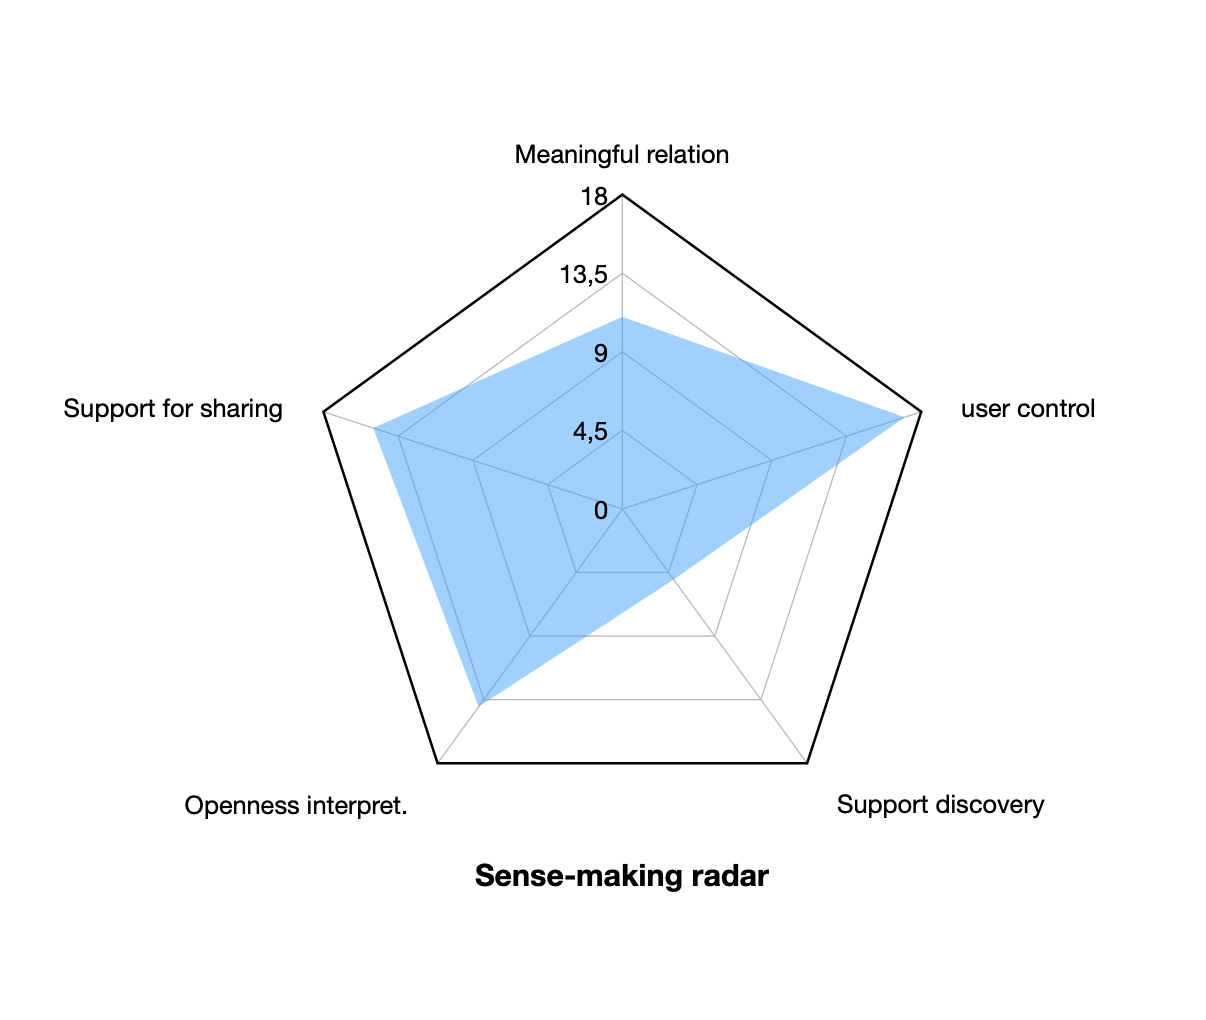
\includegraphics[width=12.5cm]{pictures/analysis/sense_radar.png}
    \caption{Sense-making radar}
\end{table}


From the radar chart 7.8, we can see \textit{User-Control} being the most fulfilled principle, counting 17 installations. \textit{Openness to interpretation} and \textit{Support for sharing} are moderately fulfilled, while \textit{Meaningful Relation} less so, and \textit{Support for Discovery} the least, counting only five principles. Looking at Table 7.6, the validity of all principles except \emph{meaningful relation with target} can be misleading or skewed due to the nine MUNCH Shadows all answering the same and therefore bringing a heavier weight to the four other principles. However, if we removed the MUNCH Shadows from this data-set, the \textit{Openness to interpretation} principle would turn from weighted green - to red. \emph{User control} and \emph{support for sharing} would still be weighted green the most, with or without MUNCH Shadows. \emph{Support for discovery} would be weighted red, with with or without MUNCH Shadows.


\section{Seeing the theories compare}
To identify the meaningful relations between visitor-experience, installation and the museum we need to put the three concepts together. As seen at the bottom of Tables 7.3, 7.5, and 7.7, the number of installations adding to the dialogic principle have been counted. This is summarised in Figure 7.2 correspondence table below. The number is the amount of installations adding to the principle, e.g. Place open 7, tell us that seven installations count the \emph{Open} principle from the Place as a Dialogue approach. In an attempt to see how the three theories relate/ compares up against each-other, it was decided to make a Heat-map based on the correspondence table. See Figure 7.3 Heat-map.

\begin{figure}[H]
    \centering
    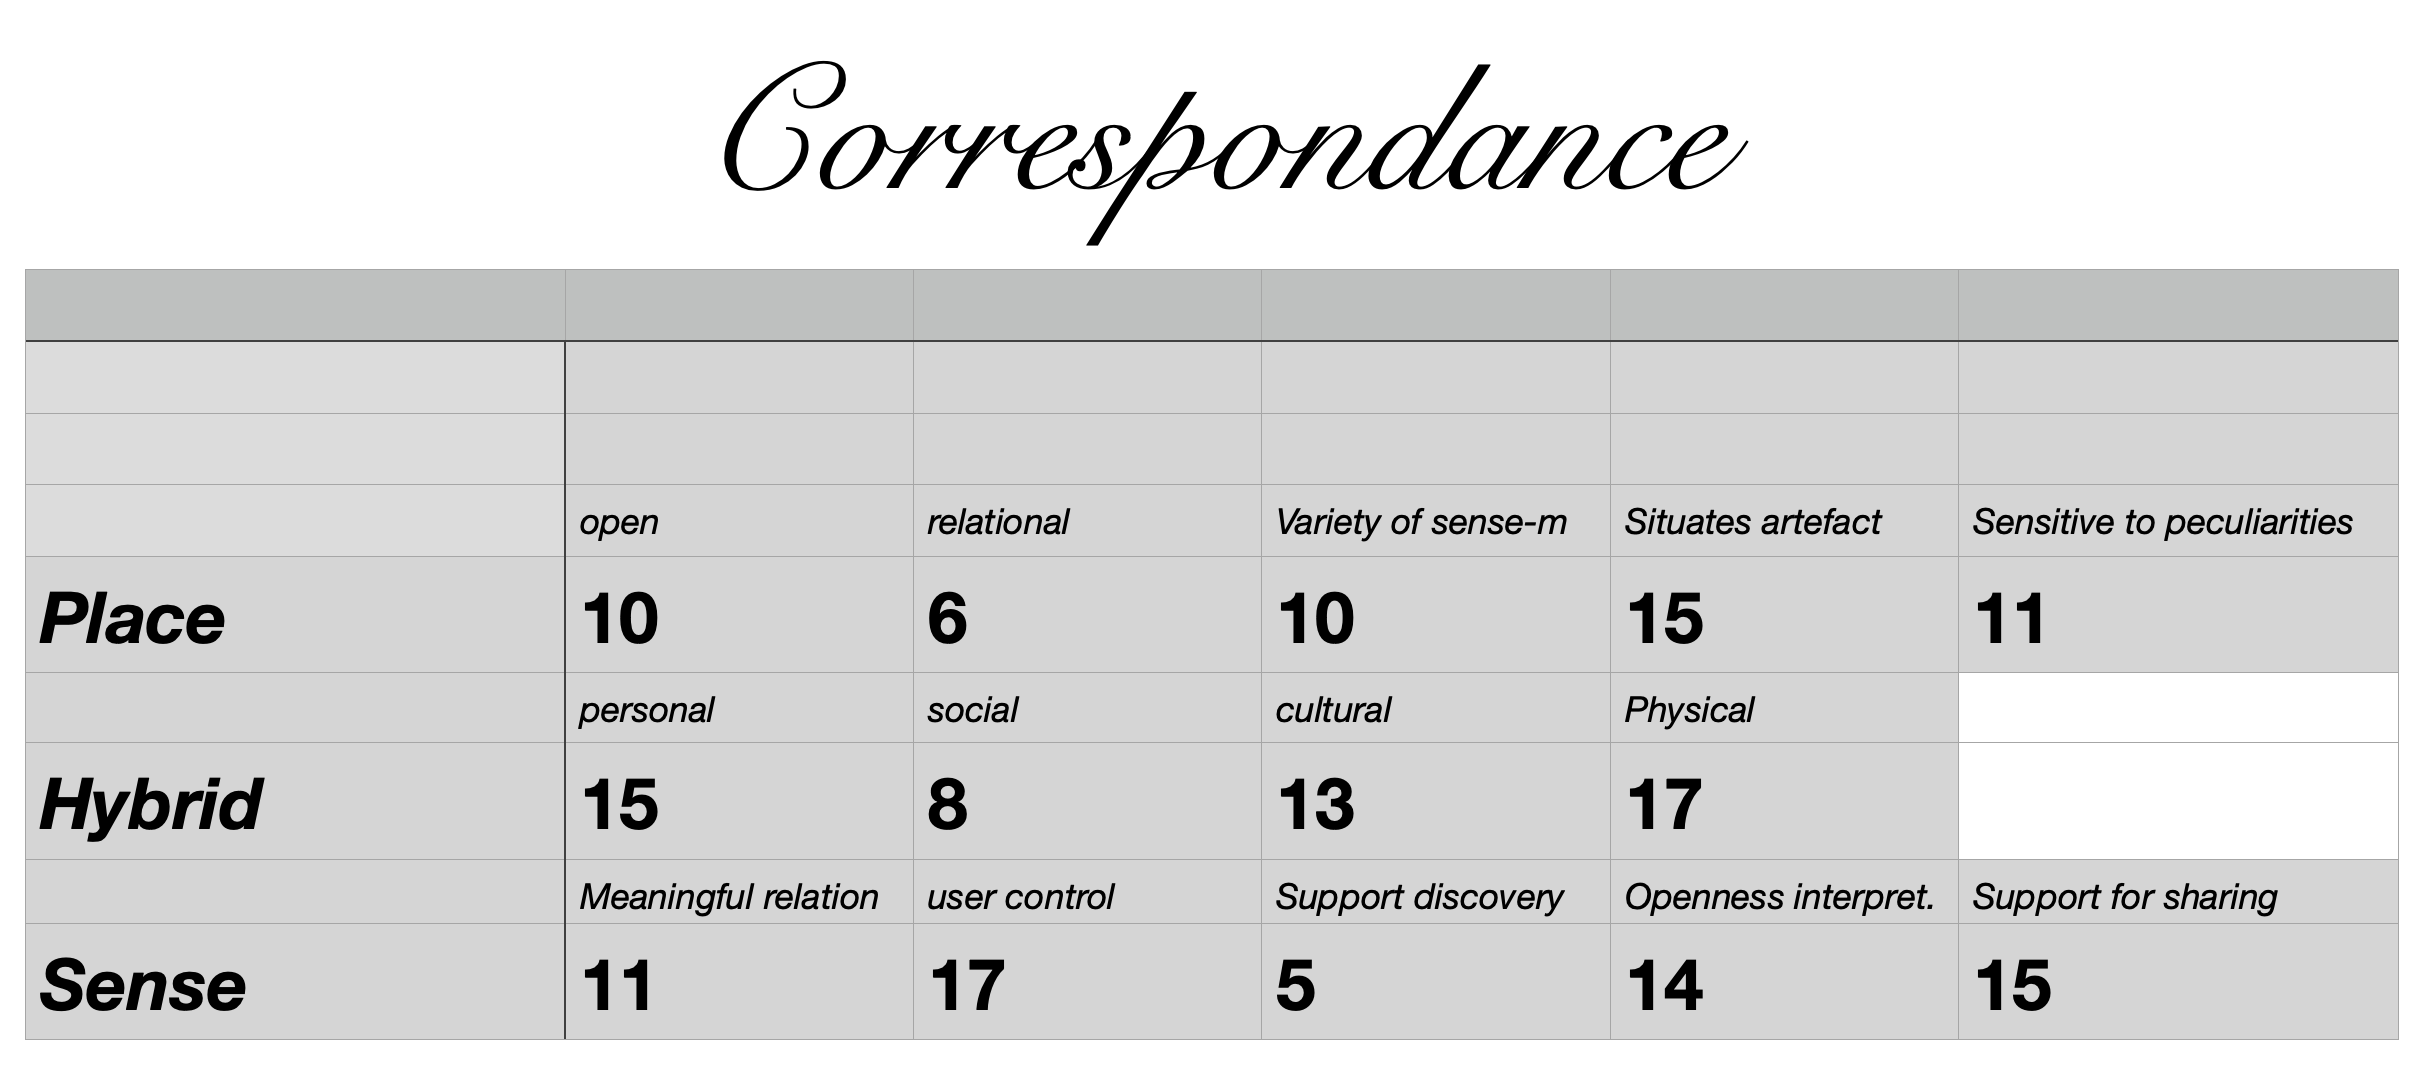
\includegraphics[width=13cm]{pictures/analysis/correspondence.png}
    \caption{Correspondence table}
\end{figure}

The categorization in Figure 7.2 Correspondence table opened up for looking at the data-set in correlation with each theory separately, while making it possible to see overall trends in the data-set across the theories. In dialogue with my supervisor, it was suggested to try heat-mapping the correspondence table, to compare the principles with the most installations up against the principles with the least. This way it would become truly explicit which principles/ dimensions are the most trending in this data-set, across the three approaches.  See Figure 7.3 for the heat-map visualisation. The heat-map is simply drawn on top of the correspondence table using a raster graphics editor app for digital painting. The principles with the highest installation-counts are coloured in red, then ranging downward from orange to yellow and green, where the blue represents the principles with the lowest installation count.

\begin{figure}[H]
    \centering
    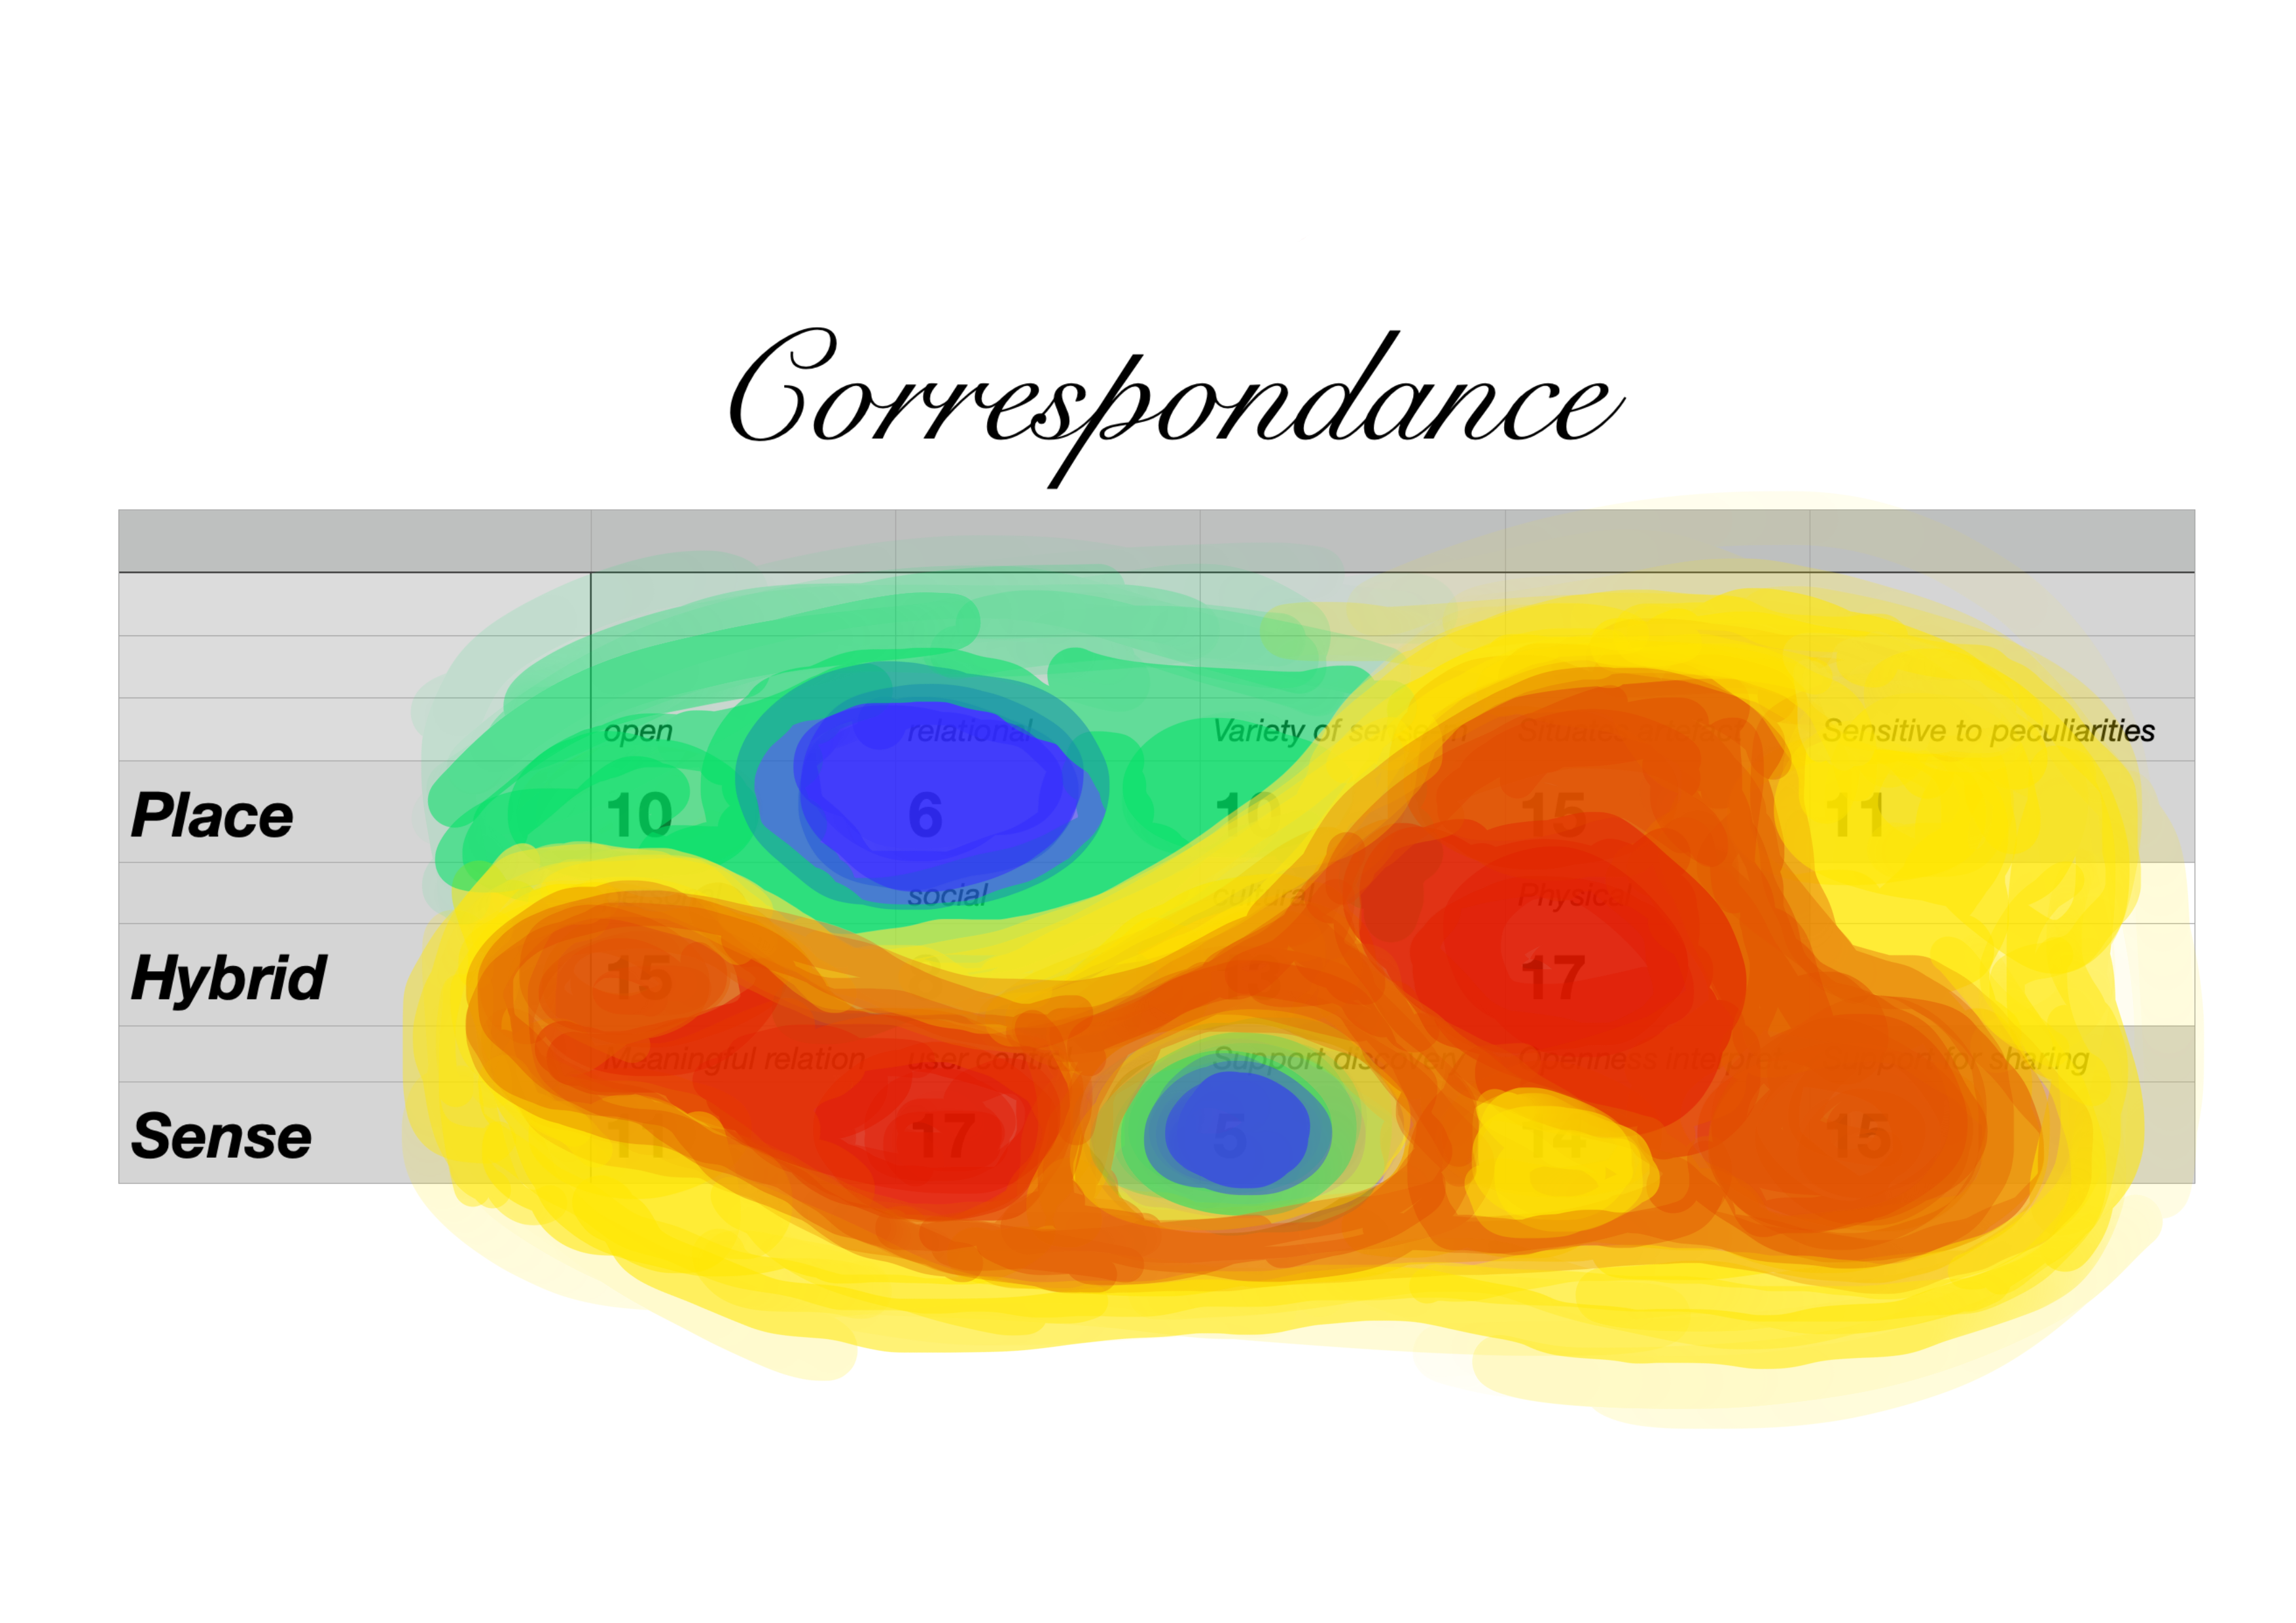
\includegraphics[width=13cm]{pictures/analysis/heat_map_new.png}
    \caption{Heat-map}
\end{figure}

The first thing we see is the warmth surrounding Sense and Hybrid, while Place generally is a little colder. The warmest principles are the Hybrid: Physical and Personal, Sense: User control and openness to interpretation, and Place: Situates artefact in narrative. The warmth could tell us that, among the installations we have analysed, there is a high degree of sense-making interactive qualities that makes the visitor engage with their surroundings. And that a high degree of museum space "hybridness" supports this engagements. However, linked to the coldness surrounding Place: relational, and Sense: support for discovery - it would mean that the visitor experience are not so much dialogic, across the installations we have analysed. In this research context, this would indicate that for the designer working to design for meaningfulness in a museum context, could lie her design efforts in enhancing dialogic visitor experiences. This could, for example, be achieved by practically using Place as a Dialogue principles to enhance the installation design.

\section{Findings}
After going through Tables 7.3-7.8, we have seen how each theoretical approach applies to the 21 installations that make up the data-set. We are aware of how the numbers of installations in one exhibition can skew the results, e.g. MUNCH Shadows. Through heat-mapping the correspondence table we have seen how the three theories compare up against each-other, and learned how to read and use the three aspects of meaningfulness together - seeing how they respectively fulfill different aspects in terms of objectifying meaningfulness as a quality that you can design for. In this research context, it will give the means to indicate how one can design for meaningfulness. 

In this next step, we are going to see how we can utilise the framework to not only make visible dialogic qualities and relations between interactive installations and visitor-experience. We are going to use the Tables 7.3, 7.5, 7.7 as the basis to identify a pattern, directly derived from each of the 21 installations. At risk of repeating myself from Chapter 4: A new way of designing for meaningfulness?, we are using Christopher Alexander's working explanation for the logic behind pattern creation: \emph{"Each one of these patterns is a morphological law, which establishes a set of relationships in space. This morphological law can always be expressed in the same general form:}

\begin{quote}
\centering $X \rightarrow r (A, B, ...)$,
\end{quote}

\emph{
which means: Within a context of type X, the Parts A, B, ... are related by the relationship r. "}\autocite[p. 90]{Alexander_book}. To apply this way of pattern-creation to our research context, we will first have to identify the "context of type x", which is the museum space and its disseminated discourse. E.g. Klimahuset disseminating the climate crisis. In our quest to answer how one can design for meaningfulness in a museum space, we seek to find dialogical relations "r" between installations and the visitor, through objectified meaningful qualities in the museum space; "(A, B, ...)". In the next section you will be presented to a list of patterns in Table 7.9. These patterns have been derived in a process where I have gone through each of the 21 installations, and used Table 7.3, 7.5, and 7.7 to "see" the specific installation in reference to itself, seeing which dimensions and principles it fulfill to guide the notion of how the visitor experience was meaningful. During this process I had a picture of the installation by my side as well, to further stimulate the memory of the installation, ref Figure 7.4. 

\begin{figure}[H]
    \centering
    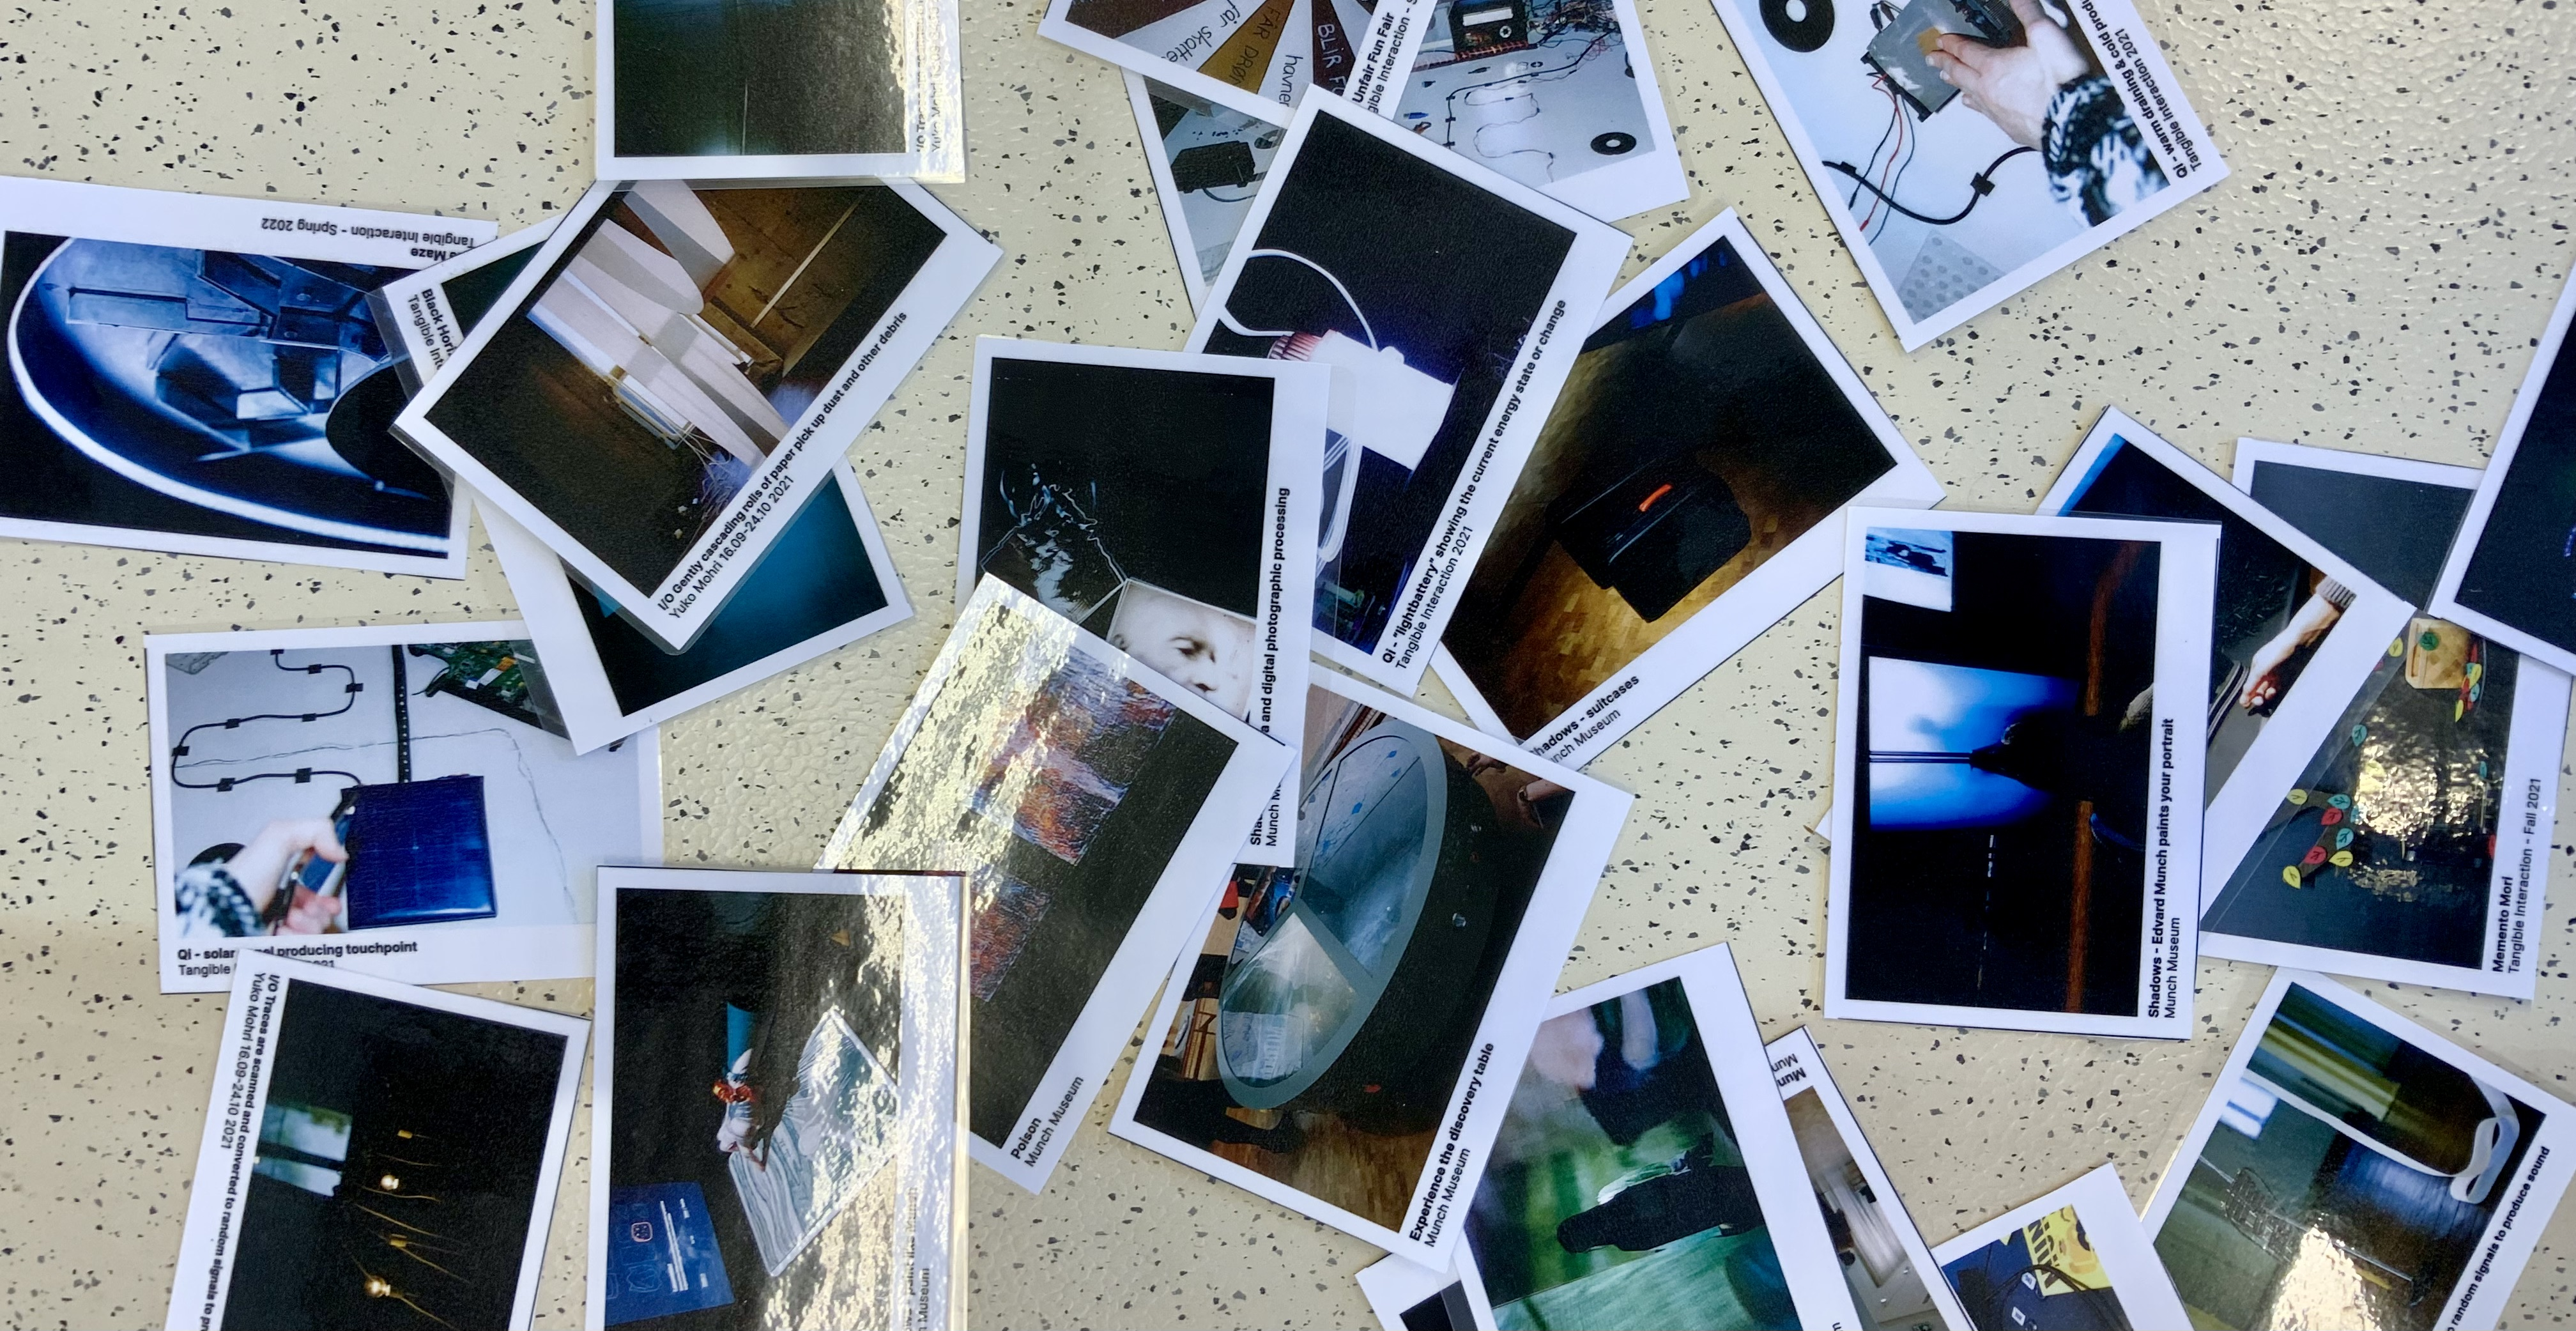
\includegraphics[width=12cm]{pictures/analysis/pictures.jpeg}
    \caption{Installation pictures}
\end{figure}

\break
Then, going through each of the 21 installations by using the pattern-logic by \autocite{Alexander_book}, I derived the patterns presented in Table 7.9. The number in Table 7.9 corresponds with the initial installation numbering in the beginning of this chapter in Table 7.2: Installations.

\subsection{Patterns}
Each pattern in Table 7.9 should be read as following:

\begin{quote}
    In the museum space, the dialogical visitor experience is meaningfully objectified by:
\end{quote}

\begin{table}[H]
\centering
\begin{tabular}{| p{0.75cm} | p{11cm}| }
\hline
\textbf{Nr} & \textbf{Pattern}\\
\hline
1 & Presenting an artefact that physically represents the exhibition topic and proposes a personalised route through the exhibition.\\
\hline
2 & Leaving the visitor to make its own way through the exhibition space.\\
\hline
3 & Having multiple interactive touchpoints with no prescribed sequence of actions, nor a defined start or end.\\
\hline
4 & Letting the visitor choose and place an interactive artefact wherever they like on the installation surface to gain access to a personalised end.\\
\hline
5 & Having multiple interactive touchpoints with no prescribed sequence of actions, nor a defined start or end.\\
\hline
6 & Letting the visitor control the installation pace.\\
\hline
7 & Making the visitor "repair" the installation by putting the interactive elements where they belong, to gain access to the end.\\
\hline
8 & Guiding two-and-two visitors through a prescribed sequence of actions, as a necessity to get the message across.\\
\hline
9 & Letting the visitor control the pacing of the information display.\\
\hline
10 & Gamifying information-claims where the visitor uses a rotating controller to give an answer, as a prerequisite to the information on the topic being displayed.\\
\hline
11 & Presenting a token that the visitor can save the choices made during the exhibition to gain access to a personalised ending.\\
\hline
12 &  Creating a distinct immersive atmosphere through video-projections and sound.\\
\hline
13 & Letting the visitor control the pacing of the interactive activity.\\
\hline
14 & Recognising the visitors presence, and generating a sound describing the visitor's situational action.\\
\hline
15 & Encouraging the visitor to take a picture of themselves, to become a part of a picture collection related to the installation theme.\\
\hline
16 & Recognising a visitors presence and action, and telling a story directly to the visitor that nearby visitors can listen in on.\\
\hline
17 & Responding to the visitors action by playing music in the nearby area.\\
\hline
18 & Responding to the visitors action, and telling a story that only the visitor can hear.\\
\hline
19 & Responding to the visitors action, and generating a distinct immersive atmosphere that describes the visitor's situational action.\\
\hline
20 & Recognising the visitors presence, and playing a video where a character speak directly to the visitor.\\
\hline
21 & Creating a distinct immersive atmosphere through video-projections and sound.\\
\hline
\end{tabular}
\caption{Findings}
\end{table}

\section{Revisiting the framework}
I will now revisit my framework and account for what I have learned by applying the framework in the analysis session. Before I introduce the revised version, I will begin by explaining the specific changes I have made to the framework based on the knowledge generated from the analysis. The framework presented in \textit{Chapter 4: A new way of designing for meaningfulness?} was built on theoretical understanding from three different approaches to place-centered design. In this research context, the three approaches fulfill three aspects of meaningfulness in a museum space. During the analysis session; plotting the installations in Tables and radar charts 7.3-7.8, heat-mapping the correspondence in Figure 7.3, and creating the patterns - the outlook of the generated insights became more clear:

\begin{itemize}
    \item Hybrid represent >> the degree of \textit{Museum space "hybridness"}
    \item Place represent >> the degree of \textit{Dialogic visitor experience}
    \item Sense represent >> the degree of \textit{Dialogic exhibition installation design}
\end{itemize}

To further explain how this new knowledge was generated through use and "talked back" informing the framework, I will use the new concept terms to explore Klimahuset, whose expository agency is to disseminate knowledge on the climate crisis. Four installations from Klimahuset have been analysed. They can numerically be traced back to the numbers 9, 10, 11, and 12, as accounted for in Table 7.2 initially in this chapter. Let's see how they map up in the application of the framework:

\begin{table}[H]
\centering 
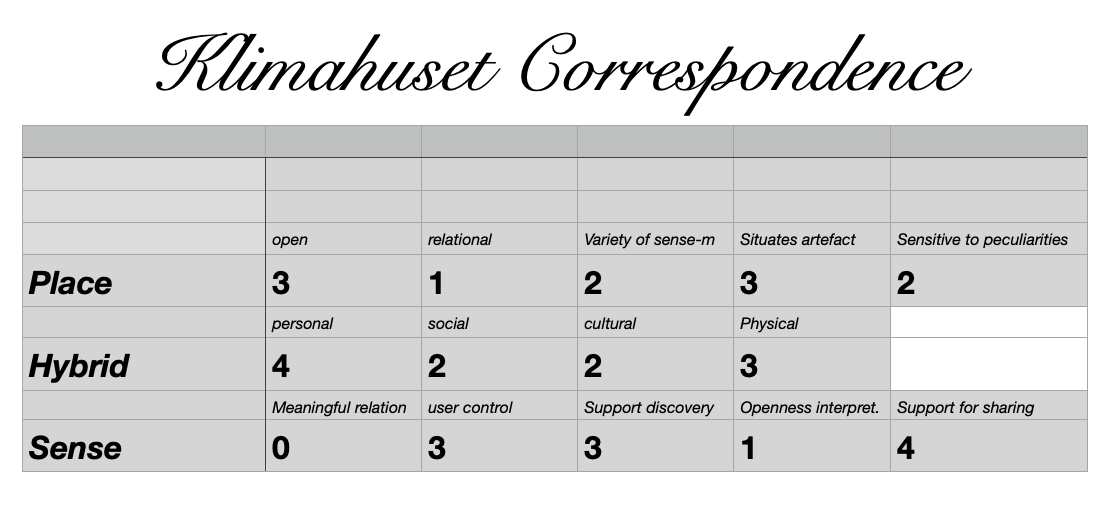
\includegraphics[width=13cm]{pictures/analysis/klimahuset_corr.png}
\caption{Klimahuset's correspondence table}
\end{table}

The first new concept term \textit{museum space "hybridness"}, derived from the Hybrid Place approach, has proved to be a valuable concept for making visible the general direction of the "hybridness" in the exhibition space. This way, one could see which dimension the exhibition leans against most - comparing it to the museum's expository agency and discourse. Klimahuset, who is disseminating knowledge on the climate crisis, and wants to increase the visitor's climate consciousness and stimulate climate action in the aftermath of the visit, should want the "hybridness" to be reflected in the exhibition "hybridness" - perhaps leaning toward the social or personal dimension. Based on the correspondence Table 7.10, I have mapped out three radars:

\begin{figure}[H]
\centering 
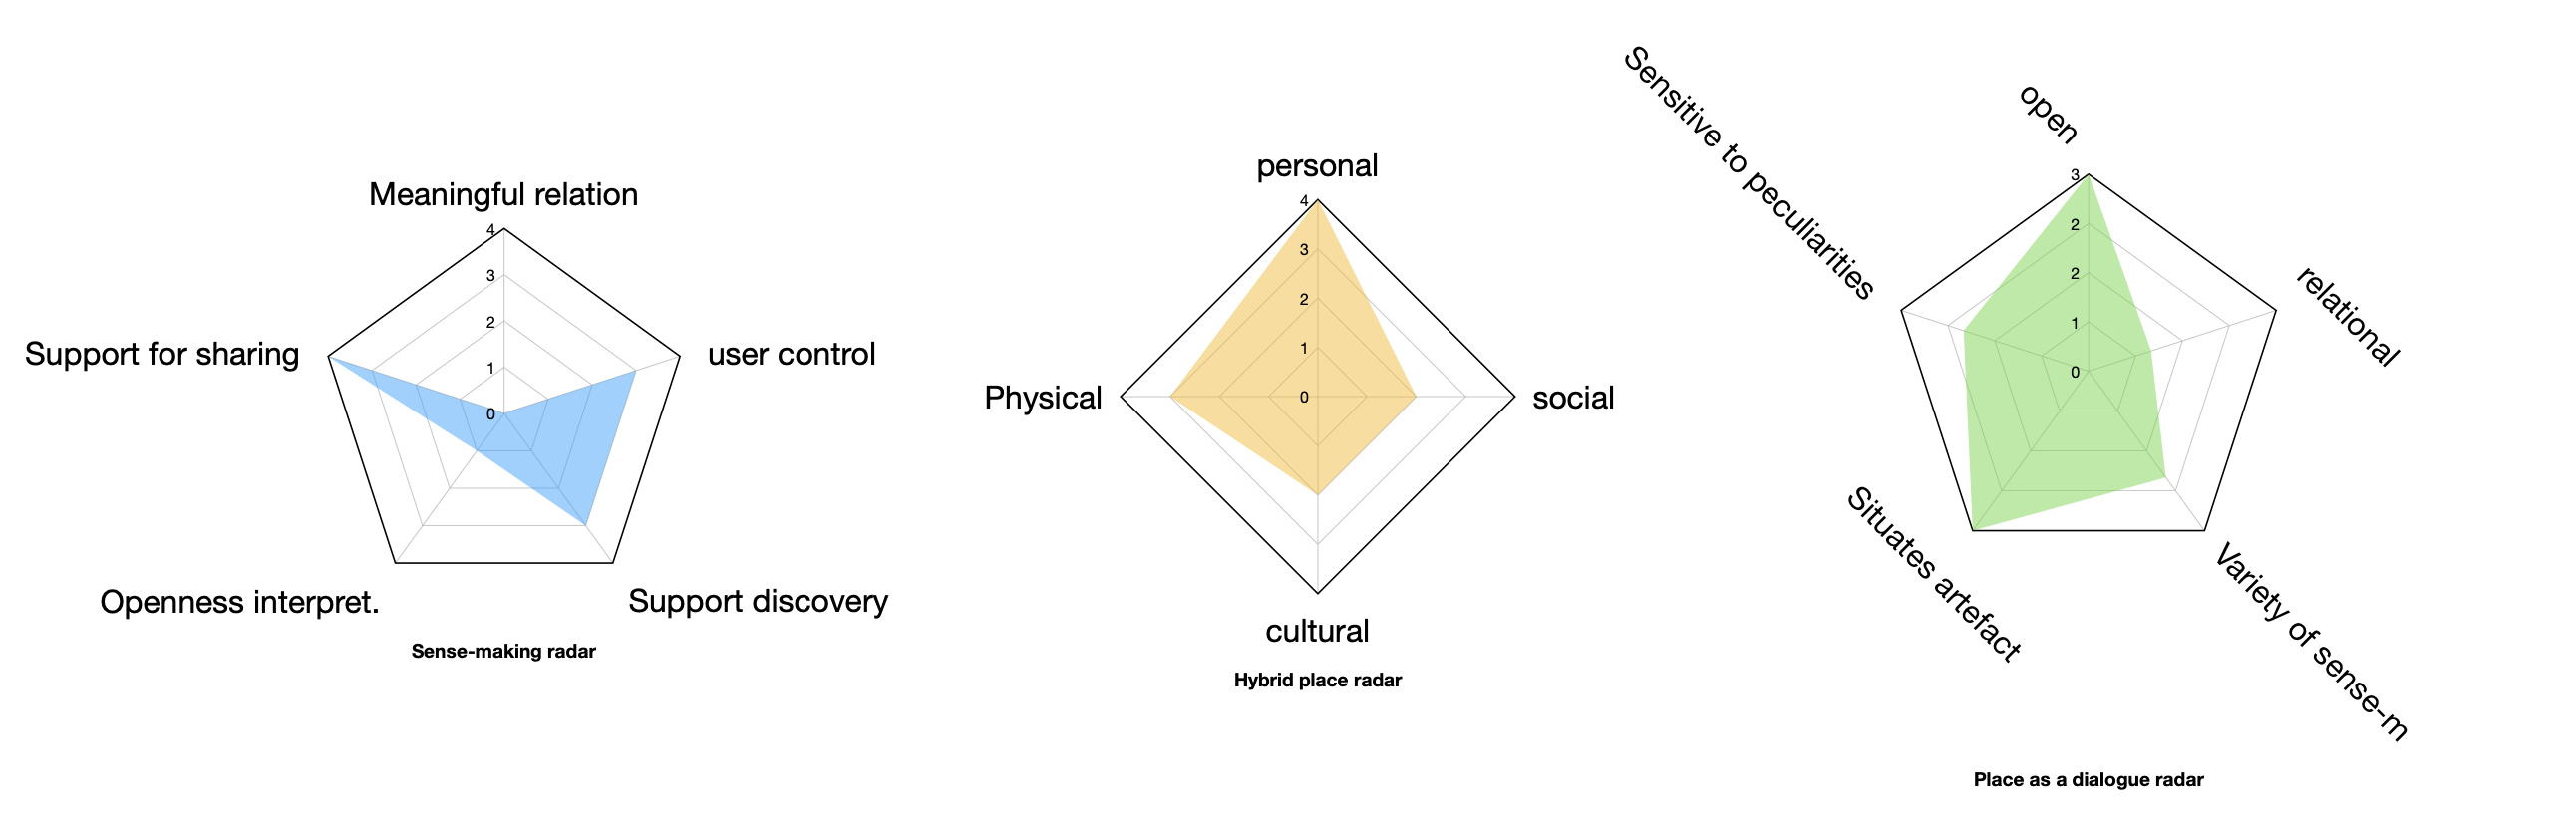
\includegraphics[width=13cm]{pictures/analysis/klimahuset_analysis_radars.png}
\caption{Klimahuset exhibition analysis}
\end{figure}

As we can see, the exhibition "hybridness" leans the most against the personal dimension, where four out of four installations count the dimension. Two installations count social and cultural, and three counts the physical dimension. This would give the museum stakeholders involved in the exhibition design, e.g., the curator, to look at the current exhibition against the museum agency and vision and from there be able to articulate a need for installations or exhibition artefacts to address the hybrid dimension direction they would like the exhibition experience to inherit. This would provide the museum stakeholders with a tool for articulating and framing a specific need and wanted direction for the exhibition based on the current state of affairs. At the same time, the designer is enabled to join the exhibition- or installation design process with more explicit constraints from the beginning and can start with conceptual work and exploration earlier.

The second new concept term \textit{Dialogic visitor experience}, derived from the Place as a dialogue approach, has proved to be a valuable concept for making visible dialogic visitor experience, rooted in the exhibition space. In the radar chart in Figure 7.5, we see how three out of four installations counts the \emph{open} and \emph{situates artefact in narrative} principle, while two installations touches upon the \emph{sensitive to the pec. of space and time} and \emph{in the centre of a variety of s.m.p.} principle.

% Wanting to get a better understanding of the visitor experience with attention to the sensory transactions and the way the experience transform in the telling (what is the things you remember), I utilise \autocite{spaceplace_ciolfi} "dialogical ontology", or as I call it, the list of place-related qualities. 


The third new concept term \textit{Dialogic exhibition and installation design}, derived from the Sense-making approach, has proved to be a valuable concept for making visible dialogic qualities in the exhibition- and installation design. In the radar chart in Figure 7.5, we see how four out of four installations count to \emph{support for sharing}, three count \emph{user control} and \textit{support for discovery}.


\begin{figure}[H]
\centering 
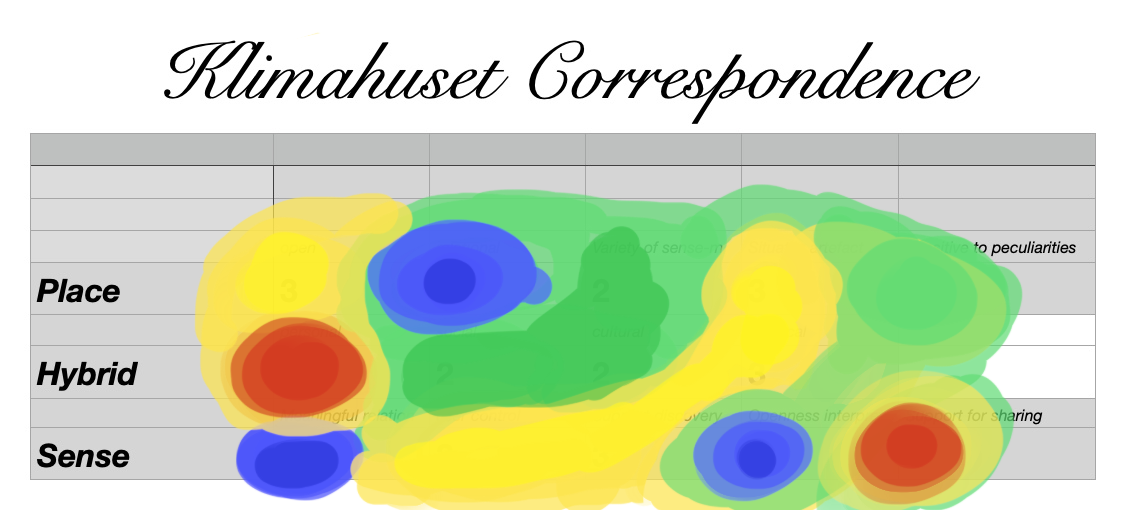
\includegraphics[width=13cm]{pictures/analysis/klimahuset_heat.png}
\caption{Heat-mapping Klimahuset's exhibition}
\end{figure}


\subsection{Revised framework}


\begin{figure}[H]
\centering 
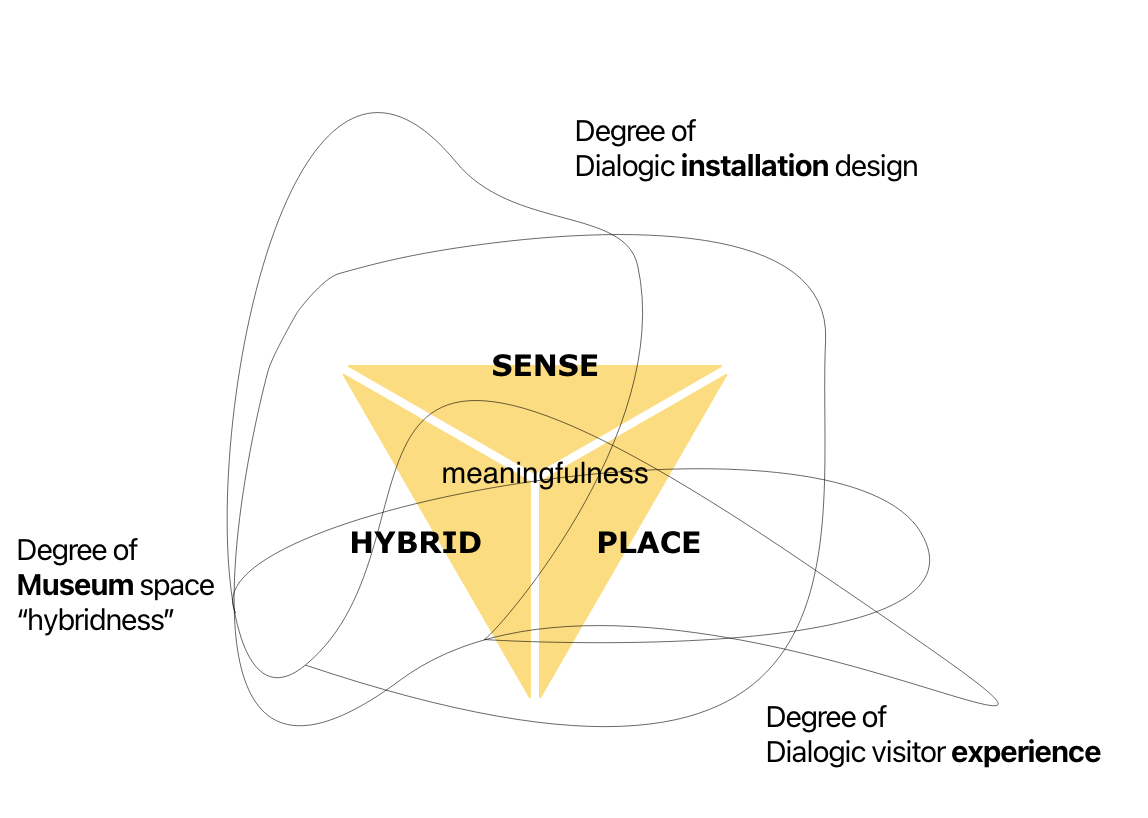
\includegraphics[width=13cm]{pictures/analysis/triangle_revised.png}
\caption{Revised version of meaningfulness triangle}
\end{figure}

